\section{Experimental Evaluation}\label{sec:experiments} 



We compare against state-of-the-art multi-matching methods %
with a focus on quantum methods. 
We consider classical works for reference. 
All experiments use Python 3.9 on an Intel Core i7-8565U CPU with 8GB RAM and the D-Wave Advantage System 4.1 (accessed via Leap 2). 
We will release our code, which is accelerated using Numba. 


\noindent\textbf{Hyperparameters.} We set $T{=}11$. %
We set the number of worst vertices $m$ to  $16 \%$ of the number of vertices $n$. 


\noindent\textbf{Quantum Comparisons.} 
The closest quantum work, Q-Match \cite{SeelbachBenkner2021}, matches only two shapes. 
We consider two adaptations to multi-matching: 1) Q-MatchV2-cc, similar to our CCuantuMM, chooses an anchor and matches the other shapes pairwise to it, implicitly enforcing cycle consistency; and 2) Q-MatchV2-nc matches all pairs of shapes directly, without guaranteed cycle consistency. 
In both cases, we use our faster implementation and adapt our energy matrix schedule, which gives significantly better results. 


\noindent\textbf{Classical Comparisons.} For reference, we also compare against the classical, non-learning-based  multi-matching state of the art: IsoMuSh~\cite{Gao2021}  and the \emph{synchronised} version of ZoomOut \cite{melzi2019zoomout}, which both guarantee vertex-wise cycle consistency across multiple shapes. 



\noindent\textbf{Evaluation Metric.} 
We evaluate the correspondences using the Princeton benchmark protocol \cite{VladimirGPCK}. 
Given the ground-truth correspondences $P_{\cal I J}^{*}$ for matching the shape $\mathcal{I}$ to $\mathcal{J}$, the error of vertex $v \in \mathcal{I}$ under our estimated matching $P_{\cal I J}$ is given by the normalised geodesic distance: 
\begin{equation}
    e_v(P_{\cal I J}) = \frac{d_\mathcal{J}^{g}(v^\top P_{\cal I J},v^\top P_{\cal I J}^{*})}{\operatorname{diam}(\mathcal{J})}, \quad
\end{equation}
where $\operatorname{diam}(\cdot)$ is the shape diameter. %
We plot the fraction of errors that is below a threshold in a percentage-of-correct-keypoints (PCK) curve, where the threshold varies along the x-axis. %
As a summary metric, we also report the area-under-the-curve (AUC) of these PCK curves. 

\noindent\textbf{Datasets.} 
The \emph{FAUST} dataset~\cite{Bogo:CVPR:2014} contains real scans of ten humans in different poses. 
We use the registration subset with ten poses for each class and downsample to $500$ vertices. 
\emph{TOSCA}~\cite{bronstein2008numerical} has $76$ shapes from eight classes of humans and animals. 
We downsample to ${\sim}1000$ vertices. 
\emph{SMAL}~\cite{Zuffi:CVPR:2017} has scans of toy animals in arbitrary poses, namely %
$41$ non-isometric shapes from five classes %
registered to the same template. 
(\textit{E.g.,} the felidae (cats) class contains scans of lions, cats, and tigers.)
We downsample to $1000$ vertices. 
We use the same number of vertices as IsoMuSh~\cite{Gao2021}, except that they use $1000$ vertices for FAUST. 



\subsection{Experiments on Real Quantum Annealer} 
\begin{figure}
    \centering
    \resizebox{0.49\linewidth}{!}{
    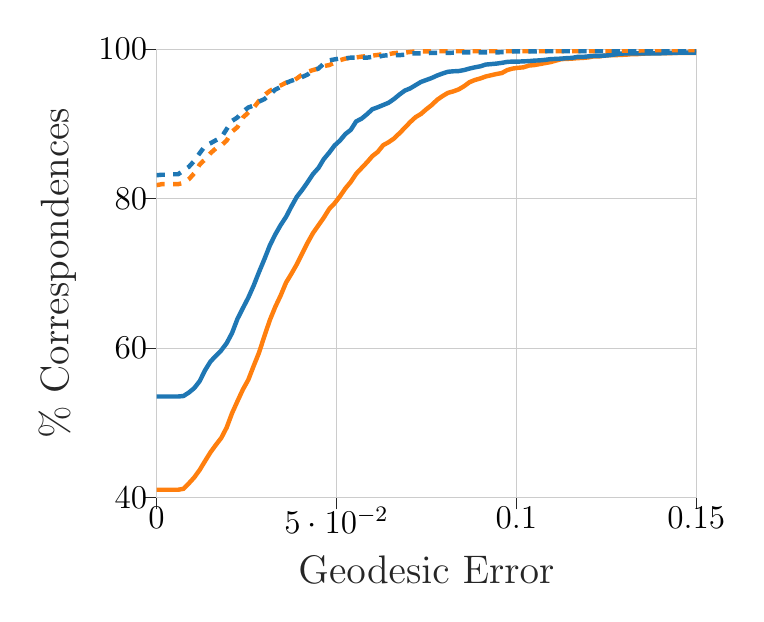
\begin{tikzpicture}

\definecolor{darkslategray38}{RGB}{38,38,38}
\definecolor{lightgray204}{RGB}{204,204,204}
\definecolor{orange}{RGB}{255,165,0}

\definecolor{darkorange25512714}{RGB}{255,127,14}
\definecolor{steelblue31119180}{RGB}{31,119,180}

\large
\begin{axis}[
axis line style={lightgray204},
legend cell align={left},
legend style={
  fill opacity=0.8,
  draw opacity=1,
  text opacity=1,
  at={(0.97,0.03)},
  anchor=south east,
  draw=lightgray204
},
xtick = {0,0.05,0.10,0.15},
tick align=outside,
tick pos=left,
x grid style={lightgray204},
xlabel=\textcolor{darkslategray38}{\Large Geodesic Error},
xticklabel style={yshift= 5pt},
xmajorgrids,
xmin=0, xmax=0.15,
xtick style={color=darkslategray38},
y grid style={lightgray204},
ylabel=\textcolor{darkslategray38}{\Large \% Correspondences},
ymajorgrids,
ymin=40, ymax=100,
ytick style={color=darkslategray38},
yticklabel style={xshift= 5pt},
]

\addplot [ultra thick, darkorange25512714]
table {%
0 41.0358565737052
0.0015 41.0358565737052
0.003 41.0358565737052
0.0045 41.0358565737052
0.006 41.0358565737052
0.0075 41.1686586985392
0.009 41.8990703851262
0.0105 42.6958831341301
0.012 43.6918990703851
0.0135 44.8871181938911
0.015 46.0491367861886
0.0165 47.0451527224436
0.018 47.9747675962815
0.0195 49.3691899070385
0.021 51.2948207171315
0.0225 52.8884462151394
0.024 54.4488711819389
0.0255 55.7436918990704
0.027 57.6029216467464
0.0285 59.3957503320053
0.03 61.6201859229748
0.0315 63.7450199203187
0.033 65.5046480743692
0.0345 67.0318725099602
0.036 68.7583001328021
0.0375 69.9535192563081
0.039 71.2151394422311
0.0405 72.675962815405
0.042 74.1035856573705
0.0435 75.398406374502
0.045 76.4276228419655
0.0465 77.456839309429
0.048 78.6188579017264
0.0495 79.3824701195219
0.051 80.3120849933599
0.0525 81.3745019920319
0.054 82.2377158034529
0.0555 83.3333333333333
0.057 84.0969455511288
0.0585 84.8605577689243
0.06 85.6905710491368
0.0615 86.2549800796813
0.063 87.1513944223108
0.0645 87.5498007968127
0.066 88.0478087649402
0.0675 88.7450199203187
0.069 89.4754316069057
0.0705 90.2390438247012
0.072 90.9030544488712
0.0735 91.3346613545817
0.075 91.9654714475432
0.0765 92.5298804780876
0.078 93.2270916334661
0.0795 93.7250996015936
0.081 94.1567065073041
0.0825 94.3559096945551
0.084 94.6215139442231
0.0855 95.0531208499336
0.087 95.5843293492696
0.0885 95.8831341301461
0.09 96.0823373173971
0.0915 96.3479415670651
0.093 96.5139442231076
0.0945 96.6799468791501
0.096 96.8127490039841
0.0975 97.2111553784861
0.099 97.4103585657371
0.1005 97.5099601593625
0.102 97.5763612217795
0.1035 97.808764940239
0.105 97.875166002656
0.1065 98.00796812749
0.108 98.140770252324
0.1095 98.273572377158
0.111 98.472775564409
0.1125 98.67197875166
0.114 98.7051792828685
0.1155 98.738379814077
0.117 98.804780876494
0.1185 98.8379814077025
0.12 98.9043824701195
0.1215 99.0371845949535
0.123 99.0371845949535
0.1245 99.136786188579
0.126 99.203187250996
0.1275 99.203187250996
0.129 99.2363877822045
0.1305 99.269588313413
0.132 99.33598937583
0.1335 99.33598937583
0.135 99.402390438247
0.1365 99.4355909694555
0.138 99.468791500664
0.1395 99.468791500664
0.141 99.468791500664
0.1425 99.468791500664
0.144 99.5019920318725
0.1455 99.5019920318725
0.147 99.5019920318725
0.1485 99.5019920318725
0.15 99.5019920318725
};
\addplot [ultra thick, steelblue31119180]
table {%
0 53.5192563081009
0.0015 53.5192563081009
0.003 53.5192563081009
0.0045 53.5192563081009
0.006 53.5192563081009
0.0075 53.5856573705179
0.009 54.0504648074369
0.0105 54.6480743691899
0.012 55.5776892430279
0.0135 57.0385126162019
0.015 58.2005312084993
0.0165 58.9641434262948
0.018 59.6945551128818
0.0195 60.6573705179283
0.021 62.0185922974768
0.0225 63.9110225763612
0.024 65.3386454183267
0.0255 66.7330677290837
0.027 68.3598937583001
0.0285 70.1859229747676
0.03 71.9123505976095
0.0315 73.738379814077
0.033 75.199203187251
0.0345 76.460823373174
0.036 77.5564409030545
0.0375 78.9508632138114
0.039 80.2456839309429
0.0405 81.1752988047809
0.042 82.2045152722444
0.0435 83.3001328021248
0.045 84.0969455511288
0.0465 85.2921646746348
0.048 86.1553784860558
0.0495 87.1181938911023
0.051 87.7822045152722
0.0525 88.6454183266932
0.054 89.2098273572377
0.0555 90.3386454183267
0.057 90.7038512616202
0.0585 91.3014608233732
0.06 91.9654714475432
0.0615 92.2310756972112
0.063 92.5298804780877
0.0645 92.8286852589641
0.066 93.3266932270916
0.0675 93.9243027888446
0.069 94.4555112881806
0.0705 94.7543160690571
0.072 95.1859229747676
0.0735 95.6175298804781
0.075 95.8831341301461
0.0765 96.1487383798141
0.078 96.4807436918991
0.0795 96.7463479415671
0.081 96.9787516600266
0.0825 97.0451527224436
0.084 97.0783532536521
0.0855 97.2111553784861
0.087 97.4103585657371
0.0885 97.5763612217795
0.09 97.7091633466136
0.0915 97.9415670650731
0.093 98.0079681274901
0.0945 98.074369189907
0.096 98.1739707835325
0.0975 98.3067729083665
0.099 98.339973439575
0.1005 98.339973439575
0.102 98.3731739707835
0.1035 98.406374501992
0.105 98.472775564409
0.1065 98.5059760956175
0.108 98.5723771580345
0.1095 98.67197875166
0.111 98.7051792828685
0.1125 98.738379814077
0.114 98.804780876494
0.1155 98.8379814077025
0.117 98.9707835325365
0.1185 98.9707835325365
0.12 99.0371845949535
0.1215 99.1035856573705
0.123 99.1035856573705
0.1245 99.136786188579
0.126 99.203187250996
0.1275 99.3027888446215
0.129 99.402390438247
0.1305 99.4355909694555
0.132 99.4355909694555
0.1335 99.4355909694555
0.135 99.4355909694555
0.1365 99.4355909694555
0.138 99.4355909694555
0.1395 99.4355909694555
0.141 99.468791500664
0.1425 99.5019920318725
0.144 99.5019920318725
0.1455 99.535192563081
0.147 99.535192563081
0.1485 99.535192563081
0.15 99.535192563081
};
\addplot [ultra thick, darkorange25512714, dashed]
table {%
0 81.8061088977424
0.0015 81.9389110225764
0.003 81.9389110225764
0.0045 81.9389110225764
0.006 81.9389110225764
0.0075 82.1049136786189
0.009 82.6029216467464
0.0105 83.3997343957503
0.012 84.5617529880478
0.0135 85.2589641434263
0.015 86.0889774236388
0.0165 86.7197875166003
0.018 87.1181938911023
0.0195 87.7822045152723
0.021 88.9774236387782
0.0225 89.5750332005312
0.024 90.8366533864542
0.0255 91.5338645418327
0.027 92.1646746347942
0.0285 93.0942895086321
0.03 93.8579017264276
0.0315 94.4223107569721
0.033 94.8207171314741
0.0345 95.1527224435591
0.036 95.5179282868526
0.0375 95.6839309428951
0.039 96.0823373173971
0.0405 96.6135458167331
0.042 96.9787516600266
0.0435 97.2111553784861
0.045 97.4103585657371
0.0465 97.7423638778221
0.048 97.875166002656
0.0495 98.207171314741
0.051 98.539176626826
0.0525 98.738379814077
0.054 98.871181938911
0.0555 98.9043824701195
0.057 99.003984063745
0.0585 99.070385126162
0.06 99.136786188579
0.0615 99.2363877822045
0.063 99.33598937583
0.0645 99.33598937583
0.066 99.468791500664
0.0675 99.535192563081
0.069 99.535192563081
0.0705 99.6347941567065
0.072 99.7011952191235
0.0735 99.7011952191235
0.075 99.7011952191235
0.0765 99.734395750332
0.078 99.734395750332
0.0795 99.734395750332
0.081 99.734395750332
0.0825 99.734395750332
0.084 99.734395750332
0.0855 99.734395750332
0.087 99.734395750332
0.0885 99.734395750332
0.09 99.734395750332
0.0915 99.734395750332
0.093 99.734395750332
0.0945 99.734395750332
0.096 99.734395750332
0.0975 99.734395750332
0.099 99.734395750332
0.1005 99.734395750332
0.102 99.734395750332
0.1035 99.734395750332
0.105 99.734395750332
0.1065 99.734395750332
0.108 99.734395750332
0.1095 99.734395750332
0.111 99.734395750332
0.1125 99.734395750332
0.114 99.734395750332
0.1155 99.734395750332
0.117 99.734395750332
0.1185 99.734395750332
0.12 99.734395750332
0.1215 99.734395750332
0.123 99.800796812749
0.1245 99.800796812749
0.126 99.800796812749
0.1275 99.800796812749
0.129 99.800796812749
0.1305 99.800796812749
0.132 99.800796812749
0.1335 99.800796812749
0.135 99.8339973439575
0.1365 99.867197875166
0.138 99.867197875166
0.1395 99.867197875166
0.141 99.867197875166
0.1425 99.867197875166
0.144 99.867197875166
0.1455 99.867197875166
0.147 99.867197875166
0.1485 99.867197875166
0.15 99.867197875166
};

\addplot [ultra thick, steelblue31119180, dashed]
table {%
0 83.1341301460823
0.0015 83.2005312084993
0.003 83.2005312084993
0.0045 83.2669322709163
0.006 83.2669322709163
0.0075 83.7649402390438
0.009 84.2629482071713
0.0105 85.0597609561753
0.012 86.0889774236388
0.0135 87.0517928286853
0.015 87.4169986719788
0.0165 87.8154050464807
0.018 88.1806108897742
0.0195 89.3094289508632
0.021 90.4050464807437
0.0225 90.8698539176627
0.024 91.6334661354582
0.0255 92.1978751660026
0.027 92.4634794156706
0.0285 92.9946879150066
0.03 93.3266932270916
0.0315 93.9243027888446
0.033 94.5883134130146
0.0345 94.9535192563081
0.036 95.4847277556441
0.0375 95.7835325365206
0.039 96.0159362549801
0.0405 96.2815405046481
0.042 96.6135458167331
0.0435 97.1779548472775
0.045 97.4103585657371
0.0465 98.074369189907
0.048 98.5059760956175
0.0495 98.6387782204515
0.051 98.7715803452855
0.0525 98.7715803452855
0.054 98.871181938911
0.0555 98.871181938911
0.057 98.871181938911
0.0585 98.871181938911
0.06 98.9707835325365
0.0615 98.9707835325365
0.063 99.136786188579
0.0645 99.203187250996
0.066 99.203187250996
0.0675 99.203187250996
0.069 99.269588313413
0.0705 99.4355909694555
0.072 99.4355909694555
0.0735 99.4355909694555
0.075 99.468791500664
0.0765 99.5019920318725
0.078 99.5019920318725
0.0795 99.5019920318725
0.081 99.5019920318725
0.0825 99.535192563081
0.084 99.535192563081
0.0855 99.5683930942895
0.087 99.5683930942895
0.0885 99.5683930942895
0.09 99.5683930942895
0.0915 99.5683930942895
0.093 99.5683930942895
0.0945 99.5683930942895
0.096 99.601593625498
0.0975 99.6347941567065
0.099 99.7011952191235
0.1005 99.7011952191235
0.102 99.7011952191235
0.1035 99.7011952191235
0.105 99.7011952191235
0.1065 99.734395750332
0.108 99.734395750332
0.1095 99.734395750332
0.111 99.734395750332
0.1125 99.734395750332
0.114 99.734395750332
0.1155 99.734395750332
0.117 99.734395750332
0.1185 99.734395750332
0.12 99.734395750332
0.1215 99.734395750332
0.123 99.734395750332
0.1245 99.734395750332
0.126 99.734395750332
0.1275 99.734395750332
0.129 99.734395750332
0.1305 99.734395750332
0.132 99.734395750332
0.1335 99.734395750332
0.135 99.734395750332
0.1365 99.734395750332
0.138 99.734395750332
0.1395 99.734395750332
0.141 99.734395750332
0.1425 99.734395750332
0.144 99.734395750332
0.1455 99.734395750332
0.147 99.734395750332
0.1485 99.734395750332
0.15 99.734395750332
};
\end{axis}

\end{tikzpicture}
}
    \resizebox{0.49\linewidth}{!}{
    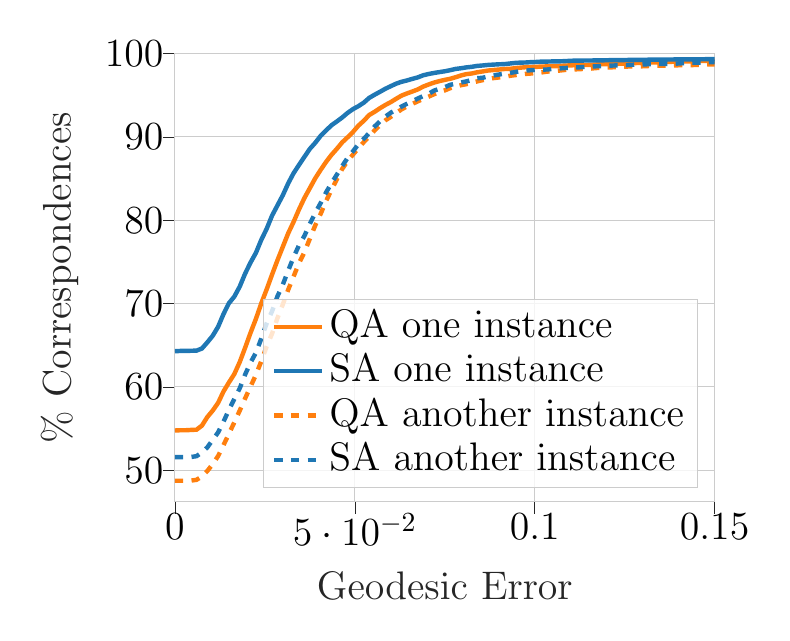
\begin{tikzpicture}

\definecolor{darkslategray38}{RGB}{38,38,38}
\definecolor{lightgray204}{RGB}{204,204,204}
\definecolor{orange}{RGB}{255,165,0}
\definecolor{darkorange25512714}{RGB}{255,127,14}
\definecolor{steelblue31119180}{RGB}{31,119,180}

\Large 
\begin{axis}[
axis line style={lightgray204},
legend cell align={left},
legend style={
  fill opacity=0.8,
  draw opacity=1,
  text opacity=1,
  at={(0.97,0.03)},
  anchor=south east,
  draw=lightgray204
},
xtick = {0,0.05,0.1,0.15},
tick align=outside,
tick pos=left,
x grid style={lightgray204},
xticklabel style={yshift= 5pt},
xlabel=\textcolor{darkslategray38}{Geodesic Error},
xmajorgrids,
xmin=0, xmax=0.15,
xtick style={color=darkslategray38},
y grid style={lightgray204},
ylabel=\textcolor{darkslategray38}{\% Correspondences},
ymajorgrids,
ymin=46.2039619300576, ymax=100,
ytick style={color=darkslategray38},
yticklabel style={xshift= 5pt},
]
\addplot [ultra thick, darkorange25512714]
table {%
0 54.763169544046
0.0015 54.7941567065073
0.003 54.7941567065073
0.0045 54.8317839752102
0.006 54.8605577689243
0.0075 55.3497122620629
0.009 56.3789287295263
0.0105 57.153607791058
0.012 58.0787959274015
0.0135 59.4510845506861
0.015 60.522355024347
0.0165 61.5316511730855
0.018 62.9681274900398
0.0195 64.6790615316512
0.021 66.4763169544046
0.0225 68.1474103585657
0.024 70.0177069499778
0.0255 71.7020805666224
0.027 73.481629039398
0.0285 75.1947764497565
0.03 76.8260292164674
0.0315 78.444001770695
0.033 79.8162903939796
0.0345 81.3036741921204
0.036 82.6715360779106
0.0375 83.8490482514387
0.039 85.0265604249668
0.0405 86.0358565737052
0.042 86.9853917662683
0.0435 87.8331119964586
0.045 88.5613103142984
0.0465 89.3426294820717
0.048 89.9513058875609
0.0495 90.5953961930057
0.051 91.3457281983178
0.0525 91.9344842850819
0.054 92.6228419654714
0.0555 93.0035413899956
0.057 93.4373616644533
0.0585 93.8291279327136
0.06 94.1722000885348
0.0615 94.572819831784
0.063 94.9513058875609
0.0645 95.2102700309872
0.066 95.4448871181939
0.0675 95.6883576803895
0.069 96.0292164674634
0.0705 96.281540504648
0.072 96.5073041168658
0.0735 96.6888003541389
0.075 96.8348826914563
0.0765 96.9654714475431
0.078 97.1536077910579
0.0795 97.3660911907924
0.081 97.5276671093404
0.0825 97.6029216467463
0.084 97.7467906153165
0.0855 97.846392208942
0.087 97.9570606463037
0.0885 98.0168216024789
0.09 98.074369189907
0.0915 98.1363435148295
0.093 98.1584772023019
0.0945 98.235945108455
0.096 98.3045595396193
0.0975 98.3554670208056
0.099 98.3820274457724
0.1005 98.3997343957503
0.102 98.435148295706
0.1035 98.4550686144311
0.105 98.4772023019035
0.1065 98.4904825143869
0.108 98.5413899955732
0.1095 98.5723771580345
0.111 98.5945108455068
0.1125 98.6033643204958
0.114 98.6188579017264
0.1155 98.6321381142098
0.117 98.6852589641434
0.1185 98.7118193891101
0.12 98.729526339088
0.1215 98.7472332890659
0.123 98.7649402390438
0.1245 98.7782204515272
0.126 98.8069942452412
0.1275 98.8424081451969
0.129 98.8733953076582
0.1305 98.8888888888889
0.132 98.9243027888446
0.1335 98.9397963700752
0.135 98.9508632138114
0.1365 98.9840637450199
0.138 99.0061974324922
0.1395 99.0239043824701
0.141 99.0393979637007
0.1425 99.0593182824258
0.144 99.0681717574147
0.1455 99.0836653386454
0.147 99.1146525011067
0.1485 99.1212926073484
0.15 99.1212926073484
};
\addlegendentry{QA one instance}
\addplot [ultra thick, steelblue31119180]
table {%
0 64.2762284196547
0.0015 64.3094289508632
0.003 64.3094289508632
0.0045 64.3315626383356
0.006 64.3470562195662
0.0075 64.601593625498
0.009 65.3386454183267
0.0105 66.1310314298362
0.012 67.211155378486
0.0135 68.738379814077
0.015 70.037627268703
0.0165 70.8277999114652
0.018 72.0274457724657
0.0195 73.5834440017707
0.021 74.9092518813634
0.0225 76.0756972111554
0.024 77.6361221779548
0.0255 78.9685701637893
0.027 80.5511288180611
0.0285 81.7795484727755
0.03 83.0101814962373
0.0315 84.4355909694555
0.033 85.6595838866755
0.0345 86.6356795042054
0.036 87.6073483842408
0.0375 88.5590969455511
0.039 89.2850818946437
0.0405 90.1195219123506
0.042 90.7613988490483
0.0435 91.3899955732625
0.045 91.8459495351926
0.0465 92.3284639220894
0.048 92.8773793714033
0.0495 93.3311199645861
0.051 93.6830455953962
0.0525 94.1057990261178
0.054 94.6746347941567
0.0555 95.0553342186808
0.057 95.4072598494909
0.0585 95.7702523240372
0.06 96.0823373173971
0.0615 96.385568835768
0.063 96.6091190792386
0.0645 96.7684816290394
0.066 96.9610447100487
0.0675 97.1336874723329
0.069 97.3882248782647
0.0705 97.5409473218237
0.072 97.6648959716688
0.0735 97.7689243027888
0.075 97.8707392651615
0.0765 97.9969012837538
0.078 98.1496237273129
0.0795 98.2293050022133
0.081 98.3355467020805
0.0825 98.4041611332447
0.084 98.5126162018592
0.0855 98.5635236830455
0.087 98.6299247454625
0.0885 98.6675520141655
0.09 98.7073926516157
0.0915 98.7250996015935
0.093 98.795927401505
0.0945 98.8689685701637
0.096 98.9065958388667
0.0975 98.9243027888445
0.099 98.966356795042
0.1005 98.9884904825143
0.102 99.0305444887117
0.1035 99.0349712262062
0.105 99.0504648074368
0.1065 99.0571049136785
0.108 99.0792386011508
0.1095 99.1146525011066
0.111 99.1456396635678
0.1125 99.1522797698095
0.114 99.1589198760512
0.1155 99.1633466135457
0.117 99.1699867197874
0.1185 99.1788401947763
0.12 99.194333776007
0.1215 99.1987605135014
0.123 99.2054006197431
0.1245 99.2120407259848
0.126 99.2275343072154
0.1275 99.2363877822044
0.129 99.2408145196988
0.1305 99.2496679946878
0.132 99.260734838424
0.1335 99.2651615759184
0.135 99.2695883134129
0.1365 99.2762284196546
0.138 99.2806551571491
0.1395 99.2939353696325
0.141 99.2939353696325
0.1425 99.2939353696325
0.144 99.3005754758742
0.1455 99.3050022133686
0.147 99.3116423196103
0.1485 99.3337760070827
0.15 99.3337760070827
};
\addlegendentry{SA one instance}
\addplot [ultra thick, darkorange25512714, dashed]
table {%
0 48.7339530765826
0.0015 48.7339530765826
0.003 48.7339530765826
0.0045 48.7516600265604
0.006 48.8468348826915
0.0075 49.2452412571934
0.009 49.904825143869
0.0105 50.7326250553342
0.012 51.6998671978752
0.0135 53.0079681274901
0.015 54.3691899070385
0.0165 55.7348384240815
0.018 57.1425409473218
0.0195 58.6077910579902
0.021 60.028773793714
0.0225 61.4320495794599
0.024 63.0787959274015
0.0255 64.8517042939353
0.027 66.3988490482514
0.0285 68.2558654271802
0.03 69.9070385126162
0.0315 71.6777335104028
0.033 73.2669322709163
0.0345 74.8583444001771
0.036 76.1620185922975
0.0375 77.7777777777778
0.039 79.3824701195219
0.0405 80.7547587428065
0.042 82.2797698096503
0.0435 83.6210712704736
0.045 84.9136786188579
0.0465 86.157591854803
0.048 87.09606020363
0.0495 87.8773793714033
0.051 88.6542718016822
0.0525 89.3758300132802
0.054 90.0553342186808
0.0555 90.7724656927844
0.057 91.4032757857459
0.0585 91.9853917662683
0.06 92.4015050907481
0.0615 92.8508189464365
0.063 93.302346170872
0.0645 93.6564851704294
0.066 93.9597166888004
0.0675 94.2585214696769
0.069 94.5573262505533
0.0705 94.8251438689686
0.072 95.1106684373617
0.0735 95.3740593182824
0.075 95.5710491367862
0.0765 95.8410801239487
0.078 96.0292164674635
0.0795 96.1974324922532
0.081 96.319167773351
0.0825 96.4873837981408
0.084 96.6533864541833
0.0855 96.8016821602479
0.087 96.9300575475874
0.0885 97.0473660911908
0.09 97.1226206285967
0.0915 97.1735281097831
0.093 97.3173970783532
0.0945 97.4037184594953
0.096 97.4789729969013
0.0975 97.5542275343072
0.099 97.6029216467463
0.1005 97.6803895528995
0.102 97.7357237715803
0.1035 97.8308986277113
0.105 97.866312527667
0.1065 97.9371403275785
0.108 98.00796812749
0.1095 98.0677290836653
0.111 98.0898627711376
0.1125 98.1274900398406
0.114 98.1562638335546
0.1155 98.1872509960158
0.117 98.2536520584329
0.1185 98.2824258521469
0.12 98.3156263833555
0.1215 98.3444001770695
0.123 98.3820274457724
0.1245 98.4152279769809
0.126 98.4395750332005
0.1275 98.444001770695
0.129 98.4528552456839
0.1305 98.4772023019035
0.132 98.5059760956175
0.1335 98.5214696768481
0.135 98.5502434705622
0.1365 98.5568835768039
0.138 98.5635236830456
0.1395 98.5834440017706
0.141 98.5989375830013
0.1425 98.6033643204957
0.144 98.6166445329791
0.1455 98.625498007968
0.147 98.6542718016821
0.1485 98.6896857016378
0.15 98.6896857016378
};
\addlegendentry{QA another instance}

\addplot [ultra thick, steelblue31119180, dashed]
table {%
0 51.5670650730412
0.0015 51.5670650730412
0.003 51.5670650730412
0.0045 51.5825586542718
0.006 51.6865869853918
0.0075 52.1359008410801
0.009 52.7379371403276
0.0105 53.643204957946
0.012 54.5374059318282
0.0135 55.8277999114653
0.015 57.2244355909694
0.0165 58.5480301018149
0.018 59.8140770252324
0.0195 61.4718902169101
0.021 62.8950863213812
0.0225 64.0925188136344
0.024 65.7835325365206
0.0255 67.6272687029659
0.027 69.0814519698982
0.0285 70.8742806551572
0.03 72.286409915892
0.0315 73.9729969012838
0.033 75.5821159805223
0.0345 77.0075254537406
0.036 78.1230633023461
0.0375 79.5683930942895
0.039 80.8676405489155
0.0405 82.0562195661797
0.042 83.3266932270916
0.0435 84.4245241257193
0.045 85.4625940681717
0.0465 86.498450641877
0.048 87.4767596281541
0.0495 88.273572377158
0.051 89.1235059760957
0.0525 89.7742363877822
0.054 90.4603806994245
0.0555 91.2439132359451
0.057 91.8680832226649
0.0585 92.4302788844621
0.06 92.8995130588756
0.0615 93.2514386896857
0.063 93.6387782204515
0.0645 93.9729969012838
0.066 94.269588313413
0.0675 94.6038069942452
0.069 94.8893315626383
0.0705 95.1571491810536
0.072 95.5444887118194
0.0735 95.7613988490483
0.075 95.9650287737937
0.0765 96.2416998671979
0.078 96.3811420982736
0.0795 96.5227976980965
0.081 96.6555998229305
0.0825 96.8238158477202
0.084 97.0340858787074
0.0855 97.0894200973882
0.087 97.2355024347056
0.0885 97.3638778220451
0.09 97.4745462594068
0.0915 97.5830013280212
0.093 97.6582558654271
0.0945 97.7733510402833
0.096 97.8906595838867
0.0975 97.9482071713147
0.099 98.0013280212483
0.1005 98.0389552899512
0.102 98.065515714918
0.1035 98.0832226648959
0.105 98.1606905710491
0.1065 98.2005312084993
0.108 98.2470119521912
0.1095 98.2868525896414
0.111 98.3134130146082
0.1125 98.3488269145639
0.114 98.3953076582558
0.1155 98.4285081894643
0.117 98.4661354581673
0.1185 98.4949092518813
0.12 98.5170429393537
0.1215 98.5546702080566
0.123 98.5812306330234
0.1245 98.5945108455068
0.126 98.6277113767153
0.1275 98.6586985391766
0.129 98.6808322266489
0.1305 98.700752545374
0.132 98.7162461266047
0.1335 98.7273129703408
0.135 98.7472332890659
0.1365 98.7627268702965
0.138 98.767153607791
0.1395 98.7915006640106
0.141 98.8379814077025
0.1425 98.8689685701637
0.144 98.8955289951305
0.1455 98.9021691013722
0.147 98.9243027888446
0.1485 98.9619300575475
0.15 98.9619300575475
};
\addlegendentry{SA another instance}
\end{axis}

\end{tikzpicture}
}
    \caption{
    PCK curves for (left) two three-shape and (right) two ten-shape instances using QA and SA. %
    In each plot, we denote one instance by normal lines and the other one by dotted lines. 
    }
    \label{fig:QPU_three_ten}
\end{figure}
We run two three-shapes and two ten-shapes experiments with FAUST on a real QPU. 
However, since our QUBO matrices are dense, we effectively need to embed a clique on the QPU. 
(The supplement contains a detailed analysis of the minor embeddings and the solution quality.) %
Hence, we test a reduced version of our method with 20 worst vertices per shape (40 virtual qubits in total), as more would worsen results significantly on current hardware. 
To compensate for this change, we use more  iterations for the ten-shape experiments. 
We use 200 anneals per QUBO, the default annealing path, and the default annealing time of $20\mu\mathit{s}$. 
As standard chain strength, we choose $1.0001$ times the largest absolute value of entries in $Q$. 
Each ten-shape experiment takes about 10 minutes of QPU time. 
In total, our results took about 30 minutes of QPU time for a total of $5.5 \cdot 10^4$ QUBOs. 
QA under these settings achieves a similar performance as SA under the same settings (Fig.~\ref{fig:QPU_three_ten}). %
As QPU time is expensive and since we have just shown that SA performs comparably to a QPU in terms of result quality, we perform the remaining experiments with SA under our default settings, on classical hardware. 
This is common practice~\cite{SeelbachBenkner2021, Arrigoni2022, Zaech_2022_CVPR } since SA is conceptually close to QA.
For additional results, including results on the new
Zephyr hardware \cite{Zephyr2021}, we refer to the supplement. 


\subsection{Comparison to Quantum and Classical SoTA} 

\begin{table}[h]
\centering

\resizebox{\linewidth}{!}{
\begin{tabular}{|c|ccc|ccc|}\hline
      & Ours            & Q-MatchV2-cc & Q-MatchV2-nc & IsoMuSh        & ZoomOut  & HKS \\ \hline\hline
FAUST & \textbf{0.989}  & 0.886        & 0.879        & \textit{0.974}          & 0.886    & 0.746\\ 
TOSCA & \textbf{0.967}  & 0.932        & 0.940        & \textit{0.952}          & 0.864    & 0.742 \\ 
SMAL  & \textit{0.866}  & 0.771        & 0.813        & \textbf{0.926}          & 0.851    & 0.544 \\ \hline 
\end{tabular}
}
\caption{AUC averaged over all classes of each dataset. For reference, we also include classical methods on the right. 
}
\label{Table:FAUST_TOSCA_SMAL}
\end{table}

\begin{figure}
   \centering
    \resizebox{\linewidth}{!}{
    \begin{tabular}{c|cccccc}
    
    \raisebox{-0.5\height}{\includegraphics[width=.18\linewidth]{figures/tosca_qual/cat0.png}}
     &
    \raisebox{-0.5\height}{\includegraphics[width=.11\linewidth]{figures/tosca_qual/cat7.png}} &
    \raisebox{-0.5\height}{\includegraphics[width=.17\linewidth]{figures/tosca_qual/cat9.png}} & 
    \raisebox{-0.5\height}{\includegraphics[width=.13\linewidth]{figures/tosca_qual/cat3.png}} &
    \raisebox{-0.5\height}{\includegraphics[width=.16\linewidth]{figures/tosca_qual/cat4.png}} & 
    \raisebox{-0.5\height}{\includegraphics[width=.11\linewidth]{figures/tosca_qual/cat5.png}} &
    \rotatebox[origin=c]{270}{Ours} \\

    \raisebox{\height}{Source}
    &
    \raisebox{-0.5\height}{\includegraphics[width=.11\linewidth]{figures/tosca_qual_isomush/cat7.png}} &
    \raisebox{-0.5\height}{\includegraphics[width=.17\linewidth]{figures/tosca_qual_isomush/cat9.png}} &
    \raisebox{-0.5\height}{\includegraphics[width=.13\linewidth]{figures/tosca_qual_isomush/cat3.png}} &
    \raisebox{-0.5\height}{\includegraphics[width=.16\linewidth]{figures/tosca_qual_isomush/cat4.png}} &
    \raisebox{-0.5\height}{\includegraphics[width=.11\linewidth]{figures/tosca_qual_isomush/cat5.png}} &
    \rotatebox[origin=c]{270}{IsoMuSh}
    
    \end{tabular}
    }


    \caption{Qualitative results on the TOSCA  \cite{bronstein2008numerical} cat class. 
    We colour a source shape %
    and transfer this colouring to target shapes via the matches estimated by our method or IsoMuSh \cite{Gao2021}. %
    } 
    \label{fig:tosca_qualitative} 
\end{figure} 


\begin{figure*}
    \centering
    
    \begin{subfigure}{0.32 \textwidth}
    \resizebox{\textwidth}{!}{
    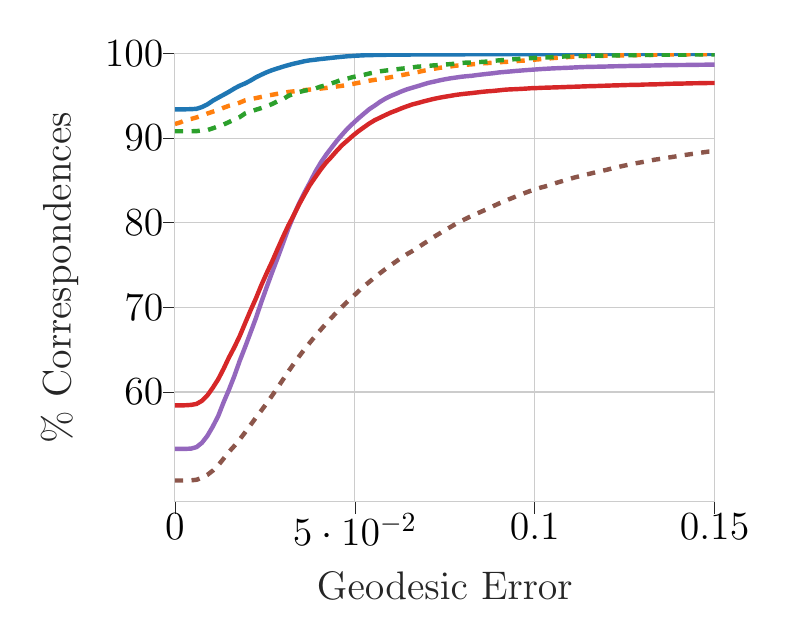
\begin{tikzpicture}

\definecolor{crimson2143940}{RGB}{214,39,40}
\definecolor{darkorange25512714}{RGB}{255,127,14}
\definecolor{darkslategray38}{RGB}{38,38,38}
\definecolor{forestgreen4416044}{RGB}{44,160,44}
\definecolor{lightgray204}{RGB}{204,204,204}
\definecolor{mediumpurple148103189}{RGB}{148,103,189}
\definecolor{sienna1408675}{RGB}{140,86,75}
\definecolor{steelblue31119180}{RGB}{31,119,180}

\Large 

\begin{axis}[
axis line style={lightgray204},
legend cell align={left},
legend style={
  fill opacity=0.8,
  draw opacity=1,
  text opacity=1,
  at={(0.97,0.03)},
  anchor=south east,
  draw=lightgray204,
},
xtick = {0,0.05,0.10,0.15},
xticklabel style={yshift= 5pt},
yticklabel style={xshift= 5pt},
ytick = {60,70,80,90,100},
tick align=outside,
tick pos=left,
x grid style={lightgray204},
xlabel=\textcolor{darkslategray38}{Geodesic Error},
xmajorgrids,
xmin=0, xmax=0.15,
xtick style={color=darkslategray38},
y grid style={lightgray204},
ylabel=\textcolor{darkslategray38}{\% Correspondences},
ymajorgrids,
ymin=47.0120185922975, ymax=100,
ytick style={color=darkslategray38},
]
\addplot [ultra thick, steelblue31119180]
table {%
0 93.4019477644976
0.0015 93.4021691013723
0.003 93.4074811863656
0.0045 93.4229747675963
0.006 93.4645861000443
0.0075 93.6702080566622
0.009 93.9803010181496
0.0105 94.4156706507304
0.012 94.7726870296591
0.0135 95.1188579017264
0.015 95.4712262062859
0.0165 95.8612217795485
0.018 96.199203187251
0.0195 96.4645861000443
0.021 96.8025675077468
0.0225 97.1790615316512
0.024 97.4922532093847
0.0255 97.7833111996458
0.027 98.0336432049579
0.0285 98.2386011509517
0.03 98.4420097388225
0.0315 98.6250553342187
0.033 98.7990261177512
0.0345 98.9389110225763
0.036 99.0894200973882
0.0375 99.1963258078796
0.039 99.2682602921646
0.0405 99.3530323151836
0.042 99.4156706507303
0.0435 99.4873837981407
0.045 99.5559982293049
0.0465 99.6177512173528
0.048 99.6757414785303
0.0495 99.7153607791058
0.051 99.7563081009296
0.0525 99.7886232846392
0.054 99.8065515714918
0.0555 99.8247011952191
0.057 99.839973439575
0.0585 99.847941567065
0.06 99.8601150951748
0.0615 99.8634351482957
0.063 99.8691899070385
0.0645 99.8747233289066
0.066 99.881584772023
0.0675 99.8851261620185
0.069 99.8860115095174
0.0705 99.8906595838866
0.072 99.893536963258
0.0735 99.8968570163789
0.075 99.9026117751217
0.0765 99.9052678176184
0.078 99.9061531651173
0.0795 99.9065958388667
0.081 99.9096945551128
0.0825 99.9163346613546
0.084 99.9196547144754
0.0855 99.9225320938468
0.087 99.9260734838424
0.0885 99.9267374944666
0.09 99.9280655157149
0.0915 99.9285081894643
0.093 99.9285081894643
0.0945 99.9293935369632
0.096 99.9318282425852
0.0975 99.9322709163346
0.099 99.9324922532093
0.1005 99.9329349269588
0.102 99.935148295706
0.1035 99.9393536963258
0.105 99.9393536963258
0.1065 99.9424524125719
0.108 99.9424524125719
0.1095 99.9431164231961
0.111 99.9446657813191
0.1125 99.945551128818
0.114 99.9459938025675
0.1155 99.9464364763169
0.117 99.9475431606906
0.1185 99.9510845506861
0.12 99.951969898185
0.1215 99.9528552456839
0.123 99.9532979194334
0.1245 99.954404603807
0.126 99.9552899513059
0.1275 99.95595396193
0.129 99.9561752988048
0.1305 99.9572819831784
0.132 99.9581673306773
0.1335 99.9586100044267
0.135 99.9586100044267
0.1365 99.9586100044267
0.138 99.9586100044267
0.1395 99.9588313413014
0.141 99.9590526781762
0.1425 99.9610447100487
0.144 99.9612660469234
0.1455 99.9612660469234
0.147 99.9612660469234
0.1485 99.9614873837981
0.15 99.9614873837981
};
\addplot [ultra thick, mediumpurple148103189]
table {%
0 53.2649402390438
0.0015 53.2689243027888
0.003 53.2749003984064
0.0045 53.3067729083665
0.006 53.4820717131474
0.0075 53.99203187251
0.009 54.804780876494
0.0105 55.898406374502
0.012 57.1294820717132
0.0135 58.7529880478088
0.015 60.2490039840637
0.0165 61.8705179282868
0.018 63.6713147410359
0.0195 65.304780876494
0.021 67.0019920318725
0.0225 68.7211155378486
0.024 70.6035856573705
0.0255 72.3824701195219
0.027 74.1314741035857
0.0285 75.8027888446215
0.03 77.5298804780876
0.0315 79.292828685259
0.033 80.8466135458167
0.0345 82.2729083665339
0.036 83.5577689243028
0.0375 84.7370517928287
0.039 85.996015936255
0.0405 87.0776892430279
0.042 88.0239043824701
0.0435 88.8545816733068
0.045 89.6812749003984
0.0465 90.4282868525897
0.048 91.1394422310757
0.0495 91.7430278884462
0.051 92.3346613545817
0.0525 92.8784860557768
0.054 93.4143426294821
0.0555 93.8346613545817
0.057 94.2908366533864
0.0585 94.6713147410359
0.06 94.9880478087649
0.0615 95.2490039840637
0.063 95.5278884462151
0.0645 95.7669322709163
0.066 95.9601593625498
0.0675 96.1454183266932
0.069 96.3446215139442
0.0705 96.5358565737051
0.072 96.6733067729083
0.0735 96.8187250996015
0.075 96.9521912350597
0.0765 97.0617529880478
0.078 97.1533864541832
0.0795 97.2470119521912
0.081 97.3147410358565
0.0825 97.3685258964142
0.084 97.4581673306772
0.0855 97.5318725099601
0.087 97.6055776892429
0.0885 97.6713147410358
0.09 97.7609561752987
0.0915 97.8147410358565
0.093 97.8705179282868
0.0945 97.9302788844621
0.096 97.9800796812748
0.0975 98.0338645418326
0.099 98.0776892430278
0.1005 98.121513944223
0.102 98.1693227091633
0.1035 98.2051792828685
0.105 98.2410358565736
0.1065 98.2689243027888
0.108 98.2948207171314
0.1095 98.3187250996015
0.111 98.3525896414342
0.1125 98.3824701195218
0.114 98.4083665338645
0.1155 98.418326693227
0.117 98.4362549800796
0.1185 98.4501992031872
0.12 98.4641434262947
0.1215 98.4860557768924
0.123 98.4980079681274
0.1245 98.5059760956175
0.126 98.5278884462151
0.1275 98.5378486055776
0.129 98.5478087649402
0.1305 98.5717131474103
0.132 98.5776892430278
0.1335 98.5896414342629
0.135 98.6055776892429
0.1365 98.6235059760955
0.138 98.6314741035856
0.1395 98.6374501992031
0.141 98.6414342629481
0.1425 98.6494023904382
0.144 98.6633466135457
0.1455 98.6673306772908
0.147 98.6752988047808
0.1485 98.6832669322708
0.15 98.6832669322708
};
\addplot [ultra thick, crimson2143940]
table {%
0 58.4123505976096
0.0015 58.4123505976096
0.003 58.4282868525896
0.0045 58.4721115537848
0.006 58.5876494023904
0.0075 58.9541832669323
0.009 59.5836653386454
0.0105 60.4840637450199
0.012 61.4820717131474
0.0135 62.7171314741036
0.015 64.0637450199203
0.0165 65.2749003984064
0.018 66.601593625498
0.0195 68.1215139442231
0.021 69.6254980079681
0.0225 71.0478087649402
0.024 72.609561752988
0.0255 74.0418326693227
0.027 75.4003984063745
0.0285 76.8665338645418
0.03 78.292828685259
0.0315 79.6573705179283
0.033 80.8705179282868
0.0345 82.1573705179283
0.036 83.3247011952191
0.0375 84.4501992031873
0.039 85.3745019920319
0.0405 86.2808764940239
0.042 87.1035856573705
0.0435 87.7828685258964
0.045 88.5119521912351
0.0465 89.1852589641434
0.048 89.7390438247012
0.0495 90.308764940239
0.051 90.8167330677291
0.0525 91.2749003984063
0.054 91.7250996015936
0.0555 92.1115537848605
0.057 92.4183266932271
0.0585 92.7270916334661
0.06 93.0239043824701
0.0615 93.2649402390438
0.063 93.5278884462151
0.0645 93.7629482071713
0.066 93.9840637450199
0.0675 94.1474103585657
0.069 94.3247011952191
0.0705 94.4860557768924
0.072 94.6414342629482
0.0735 94.7729083665338
0.075 94.8904382470119
0.0765 94.9920318725099
0.078 95.1035856573704
0.0795 95.1872509960159
0.081 95.2609561752987
0.0825 95.3227091633465
0.084 95.4003984063744
0.0855 95.4760956175298
0.087 95.5358565737051
0.0885 95.5796812749003
0.09 95.6434262948206
0.0915 95.715139442231
0.093 95.7589641434262
0.0945 95.7828685258963
0.096 95.816733067729
0.0975 95.8505976095617
0.099 95.8984063745019
0.1005 95.9163346613545
0.102 95.9482071713147
0.1035 95.9661354581673
0.105 95.9880478087649
0.1065 96.00796812749
0.108 96.0258964143426
0.1095 96.0577689243027
0.111 96.0737051792828
0.1125 96.0956175298804
0.114 96.121513944223
0.1155 96.1414342629481
0.117 96.1553784860557
0.1185 96.1812749003983
0.12 96.1992031872509
0.1215 96.2231075697211
0.123 96.2390438247011
0.1245 96.2609561752987
0.126 96.2808764940238
0.1275 96.2908366533864
0.129 96.3007968127489
0.1305 96.3346613545816
0.132 96.3446215139441
0.1335 96.3565737051792
0.135 96.3784860557768
0.1365 96.4043824701195
0.138 96.4262948207171
0.1395 96.4402390438246
0.141 96.4482071713147
0.1425 96.4661354581673
0.144 96.4820717131473
0.1455 96.4900398406374
0.147 96.503984063745
0.1485 96.51593625498
0.15 96.51593625498
};

\addplot [ultra thick,dashed, darkorange25512714]
table {%
0 91.6682988047811
0.0015 91.8573559096949
0.003 92.1534072598499
0.0045 92.2699092518816
0.006 92.4444147853034
0.0075 92.6561049136786
0.009 92.9077742363879
0.0105 93.1210084108013
0.012 93.3243311199647
0.0135 93.5868308986276
0.015 93.820584329349
0.0165 93.9781297034086
0.018 94.1964696768483
0.0195 94.4627162461269
0.021 94.6034532979197
0.0225 94.7307100486944
0.024 94.866814962373
0.0255 95.0051606905713
0.027 95.1204501992035
0.0285 95.2372828685262
0.03 95.3412611775124
0.0315 95.4511212926075
0.033 95.5294431164233
0.0345 95.6038857901726
0.036 95.6777923860115
0.0375 95.7374249667994
0.039 95.7899269588312
0.0405 95.8569738822487
0.042 95.9315214696767
0.0435 96.0127498893314
0.045 96.1053359893757
0.0465 96.1861797255421
0.048 96.2939172200086
0.0495 96.4090708277998
0.051 96.5369482071712
0.0525 96.667708277999
0.054 96.7856184152279
0.0555 96.8869433377599
0.057 96.9861580345284
0.0585 97.0896980965028
0.06 97.2038640991587
0.0615 97.3278587870737
0.063 97.4450053120849
0.0645 97.5617963700753
0.066 97.6993984063747
0.0675 97.8068924302792
0.069 97.9534856131036
0.0705 98.0742872952638
0.072 98.1945254537411
0.0735 98.304020362993
0.075 98.389926516158
0.0765 98.4715276671097
0.078 98.5557777777782
0.0795 98.6202328463926
0.081 98.6725170429397
0.0825 98.7215692784422
0.084 98.7778260292168
0.0855 98.8353948649849
0.087 98.8738255865432
0.0885 98.9146892430284
0.09 98.9640730411692
0.0915 99.0067091633472
0.093 99.0378357680395
0.0945 99.0886843736173
0.096 99.1400743691906
0.0975 99.1785024347063
0.099 99.2314125719351
0.1005 99.2930987162467
0.102 99.3449207613994
0.1035 99.395184594954
0.105 99.457755201417
0.1065 99.503370075255
0.108 99.5598401947769
0.1095 99.5897419212044
0.111 99.6271522797702
0.1125 99.6498583444005
0.114 99.6764285081898
0.1155 99.6943700752548
0.117 99.7095489154496
0.1185 99.7231677733513
0.12 99.737783089863
0.1215 99.7508472775567
0.123 99.7730004426739
0.1245 99.786519698982
0.126 99.7996024789731
0.1275 99.8113652058434
0.129 99.8235599822932
0.1305 99.8379654714476
0.132 99.8480455953963
0.1335 99.8579132359452
0.135 99.8658946436477
0.1365 99.8769853917663
0.138 99.8854218680833
0.1395 99.8899667994688
0.141 99.8975090748119
0.1425 99.907606020363
0.144 99.9174860557769
0.1455 99.920591854803
0.147 99.924586542718
0.1485 99.9319065958389
0.15 99.9319065958389
};
\addplot [ultra thick,dashed, forestgreen4416044]
table {%
0 90.8100929614874
0.0015 90.8100929614874
0.003 90.8100929614874
0.0045 90.8123063302346
0.006 90.8277999114652
0.0075 90.9074811863656
0.009 90.9473218238158
0.0105 91.1598052235503
0.012 91.3877822045153
0.0135 91.6046923417441
0.015 91.8946436476317
0.0165 92.2000885347499
0.018 92.4833997343958
0.0195 92.921646746348
0.021 93.149623727313
0.0225 93.3532536520584
0.024 93.5502434705622
0.0255 93.7782204515272
0.027 94.0283311199645
0.0285 94.3470562195661
0.03 94.5861000442673
0.0315 94.9933598937582
0.033 95.2324037184595
0.0345 95.4493138556883
0.036 95.6086764054891
0.0375 95.7259849490926
0.039 95.8676405489155
0.0405 96.091190792386
0.042 96.2571934484285
0.0435 96.4696768481629
0.045 96.6865869853918
0.0465 96.9389110225763
0.048 97.0451527224436
0.0495 97.2244355909695
0.051 97.3417441345728
0.0525 97.476759628154
0.054 97.6361221779548
0.0555 97.7711376715361
0.057 97.8950863213812
0.0585 97.9814077025233
0.06 98.0544488711819
0.0615 98.1319167773351
0.063 98.2115980522355
0.0645 98.273572377158
0.066 98.3554670208056
0.0675 98.4484285081895
0.069 98.4882691456396
0.0705 98.5369632580787
0.072 98.6033643204957
0.0735 98.6321381142098
0.075 98.6963258078795
0.0765 98.7450199203187
0.078 98.8069942452412
0.0795 98.8778220451527
0.081 98.9243027888446
0.0825 98.9420097388224
0.084 98.9707835325365
0.0855 99.0128375387339
0.087 99.0548915449313
0.0885 99.1367861885789
0.09 99.1899070385125
0.0915 99.2386011509517
0.093 99.2961487383797
0.0945 99.327135900841
0.096 99.3714032757857
0.0975 99.422310756972
0.099 99.4532979194333
0.1005 99.4975652943779
0.102 99.5130588756086
0.1035 99.5396193005754
0.105 99.5706064630366
0.1065 99.6170872067285
0.108 99.6436476316953
0.1095 99.6702080566622
0.111 99.6857016378928
0.1125 99.7100486941123
0.114 99.7100486941123
0.1155 99.7211155378485
0.117 99.7410358565736
0.1185 99.7521027003098
0.12 99.7609561752987
0.1215 99.7675962815404
0.123 99.7720230190348
0.1245 99.7786631252766
0.126 99.7919433377599
0.1275 99.8007968127489
0.129 99.8140770252323
0.1305 99.8185037627268
0.132 99.8339973439574
0.1335 99.8428508189463
0.135 99.8517042939353
0.1365 99.8517042939353
0.138 99.8561310314297
0.1395 99.8561310314297
0.141 99.8627711376714
0.1425 99.8716246126604
0.144 99.8782647189021
0.1455 99.887118193891
0.147 99.8893315626383
0.1485 99.8937583001328
0.15 99.8937583001328
};

\addplot [ultra thick,dashed, sienna1408675]
table {%
0 49.5334218680832
0.0015 49.5356352368305
0.003 49.5374059318282
0.0045 49.5542275343072
0.006 49.622399291722
0.0075 49.852810978309
0.009 50.1963258078796
0.0105 50.6945551128818
0.012 51.315183709606
0.0135 52.1086764054892
0.015 52.9134572819832
0.0165 53.6142098273572
0.018 54.3846834882691
0.0195 55.2233289065958
0.021 56.0903054448871
0.0225 56.9612660469234
0.024 57.7932713590084
0.0255 58.6648959716689
0.027 59.566401062417
0.0285 60.4922532093847
0.03 61.4444444444444
0.0315 62.4065958388667
0.033 63.3114209827357
0.0345 64.199203187251
0.036 65.0396193005755
0.0375 65.8306772908366
0.039 66.6102257636122
0.0405 67.3461708720673
0.042 68.0745905267818
0.0435 68.7605135015494
0.045 69.4428950863214
0.0465 70.083222664896
0.048 70.6945551128818
0.0495 71.2870739265162
0.051 71.8893315626383
0.0525 72.4814077025232
0.054 73.0004426737494
0.0555 73.535192563081
0.057 74.037627268703
0.0585 74.5216910137229
0.06 74.9820717131474
0.0615 75.4342629482072
0.063 75.8875608676405
0.0645 76.2915006640106
0.066 76.6540504648074
0.0675 77.0644090305445
0.069 77.4891544931385
0.0705 77.8853474988933
0.072 78.3317839752103
0.0735 78.720008853475
0.075 79.1108897742364
0.0765 79.4692341744135
0.078 79.8530323151837
0.0795 80.196768481629
0.081 80.5013280212483
0.0825 80.8123063302346
0.084 81.0967242142541
0.0855 81.3773793714033
0.087 81.6624612660469
0.0885 81.9654714475432
0.09 82.2633908809208
0.0915 82.5190349712262
0.093 82.7983621071271
0.0945 83.0542275343072
0.096 83.3162903939796
0.0975 83.5564409030545
0.099 83.7937140327579
0.1005 84.006418769367
0.102 84.1907923860115
0.1035 84.359229747676
0.105 84.5805666223993
0.1065 84.7746790615317
0.108 84.9643647631696
0.1095 85.1562638335547
0.111 85.3417441345728
0.1125 85.5017706949978
0.114 85.6648959716689
0.1155 85.8083222664896
0.117 85.967242142541
0.1185 86.1157591854803
0.12 86.2540947321824
0.1215 86.421646746348
0.123 86.566401062417
0.1245 86.7144754316069
0.126 86.8446215139442
0.1275 86.9805223550244
0.129 87.0969455511288
0.1305 87.2149181053564
0.132 87.3339973439575
0.1335 87.4619300575476
0.135 87.55201416556
0.1365 87.6613545816733
0.138 87.7543160690571
0.1395 87.859229747676
0.141 87.9619300575476
0.1425 88.0537848605578
0.144 88.1436476316954
0.1455 88.2392651615759
0.147 88.3286852589641
0.1485 88.4163346613546
0.15 88.4163346613546
};
\end{axis}

\end{tikzpicture}

     }
     \caption{FAUST \cite{Bogo:CVPR:2014}}
     \label{fig:FAUSTquant}
    \end{subfigure}
    \begin{subfigure}{0.32 \textwidth}
    \resizebox{\textwidth}{!}{
    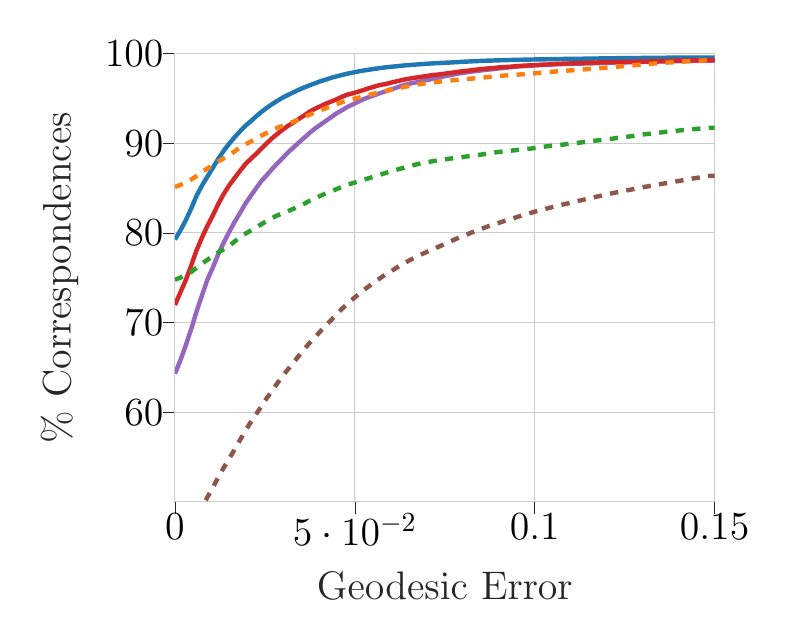
\begin{tikzpicture}

\definecolor{crimson2143940}{RGB}{214,39,40}
\definecolor{darkorange25512714}{RGB}{255,127,14}
\definecolor{darkslategray38}{RGB}{38,38,38}
\definecolor{forestgreen4416044}{RGB}{44,160,44}
\definecolor{lightgray204}{RGB}{204,204,204}
\definecolor{mediumpurple148103189}{RGB}{148,103,189}
\definecolor{sienna1408675}{RGB}{140,86,75}
\definecolor{steelblue31119180}{RGB}{31,119,180}

\Large
\begin{axis}[
axis line style={lightgray204},
legend cell align={left},
legend style={
  fill opacity=0.8,
  draw opacity=1,
  text opacity=1,
  at={(0.97,0.03)},
  anchor=south east,
  draw=lightgray204
},
xtick = {0,0.05,0.1,0.15},
ytick = {60,70,80,90,100},
xticklabel style={yshift= 5pt},
yticklabel style={xshift= 5pt},
tick align=outside,
tick pos=left,
x grid style={lightgray204},
xlabel=\textcolor{darkslategray38}{Geodesic Error},
xmajorgrids,
xmin=0, xmax=0.15,
xtick style={color=darkslategray38},
y grid style={lightgray204},
ylabel=\textcolor{darkslategray38}{\% Correspondences},
ymajorgrids,
ymin= 50, ymax=100,
ytick style={color=darkslategray38}
]
\addplot [ultra thick, steelblue31119180]
table {%
0 79.259936244157
0.0015 80.2546927190107
0.003 81.3942429041723
0.0045 82.6937871953191
0.006 84.1289444123709
0.0075 85.2643642610836
0.009 86.2596260731504
0.0105 87.2244456984884
0.012 88.2287142779153
0.0135 89.1263145056084
0.015 89.912063593532
0.0165 90.6263850703459
0.018 91.2802914141005
0.0195 91.9036651613743
0.021 92.4202388987404
0.0225 92.9678455102713
0.024 93.4733600323674
0.0255 93.9332163410713
0.027 94.3509251641448
0.0285 94.7296816403578
0.03 95.0920428723022
0.0315 95.394873598893
0.033 95.6826766799424
0.0345 95.9700026576032
0.036 96.2270097894923
0.0375 96.4681458009723
0.039 96.6872170004125
0.0405 96.9175424967315
0.042 97.0989982292176
0.0435 97.2983474598748
0.045 97.4591159297782
0.0465 97.6116270031478
0.048 97.7619371684585
0.0495 97.881912065686
0.051 97.9980282236704
0.0525 98.1076311552515
0.054 98.1994460634578
0.0555 98.2892551731614
0.057 98.3701331971687
0.0585 98.4542627317001
0.06 98.5189970370577
0.0615 98.5771012635562
0.063 98.6394390304672
0.0645 98.6932273876752
0.066 98.7369489205214
0.0675 98.7854239862609
0.069 98.8245478455438
0.0705 98.873118699513
0.072 98.9066737102316
0.0735 98.9384553344556
0.075 98.9697487905415
0.0765 98.9962479562827
0.078 99.0352358102711
0.0795 99.0656844316171
0.081 99.0961993562425
0.0825 99.1302661592989
0.084 99.1566718196572
0.0855 99.1827486340621
0.087 99.2016446313698
0.0885 99.2217466013697
0.09 99.2412888966924
0.0915 99.2582537266746
0.093 99.2753107983538
0.0945 99.2906504576653
0.096 99.3013580714801
0.0975 99.3145625006333
0.099 99.3279364112699
0.1005 99.340164586834
0.102 99.3506096501869
0.1035 99.3590519104526
0.105 99.3715491809408
0.1065 99.3830608925325
0.108 99.3928520604707
0.1095 99.4037430114886
0.111 99.4114862177474
0.1125 99.4159483437188
0.114 99.421770265621
0.1155 99.4336487819992
0.117 99.4420542960291
0.1185 99.4531100864898
0.12 99.4606389515544
0.1215 99.4708922999636
0.123 99.4788171906107
0.1245 99.4875362269393
0.126 99.4942635500861
0.1275 99.497921276865
0.129 99.5011325668775
0.1305 99.5081798075421
0.132 99.5127887076305
0.1335 99.5188497580933
0.135 99.5284871150723
0.1365 99.5314209716611
0.138 99.5338169090898
0.1395 99.5387926599573
0.141 99.5420072671322
0.1425 99.5451322261887
0.144 99.5488951860057
0.1455 99.5515102278895
0.147 99.5550279355013
0.1485 99.5580227067586
0.15 99.5580227067586
};
\addplot [ultra thick, mediumpurple148103189]
table {%
0 64.2973839234925
0.0015 65.775856259235
0.003 67.4445688326788
0.0045 69.240256672839
0.006 71.218405996147
0.0075 73.0099456313324
0.009 74.7577205369642
0.0105 76.1034586951531
0.012 77.5804455410408
0.0135 78.8752247739303
0.015 80.0427272468615
0.0165 81.1601935596876
0.018 82.1668562930586
0.0195 83.1986083789964
0.021 84.0813298801088
0.0225 84.9313787912834
0.024 85.7679438649629
0.0255 86.418133856639
0.027 87.1161054511011
0.0285 87.7619766875625
0.03 88.3654140175797
0.0315 88.9982345456972
0.033 89.5384827926116
0.0345 90.0897950218278
0.036 90.6299579985702
0.0375 91.1704466056157
0.039 91.6558211080978
0.0405 92.0704572123684
0.042 92.4971177263102
0.0435 92.9221230315245
0.045 93.3532955181705
0.0465 93.6874532865856
0.048 94.0568555431156
0.0495 94.327971266388
0.051 94.6345545228461
0.0525 94.918910763848
0.054 95.1463321490961
0.0555 95.3585042637245
0.057 95.578584604219
0.0585 95.7750375151779
0.06 95.997314057124
0.0615 96.1791731239714
0.063 96.3961663411008
0.0645 96.5589010622758
0.066 96.7066394940833
0.0675 96.8105090168199
0.069 96.9631729428548
0.0705 97.0733198161283
0.072 97.2137271868706
0.0735 97.3418646625049
0.075 97.47759555696
0.0765 97.5830864909731
0.078 97.7097410187181
0.0795 97.8123107583382
0.081 97.8946482056779
0.0825 97.9797663604946
0.084 98.0544784639896
0.0855 98.1361837005699
0.087 98.2038394226105
0.0885 98.2544927160267
0.09 98.3383160771282
0.0915 98.395941783012
0.093 98.4679471422518
0.0945 98.5160039002204
0.096 98.5747795144134
0.0975 98.6209396067986
0.099 98.6480119094453
0.1005 98.6962975033298
0.102 98.7415254935252
0.1035 98.7554199101652
0.105 98.7724814665277
0.1065 98.814751122364
0.108 98.8291167240539
0.1095 98.8407758240957
0.111 98.8533369304132
0.1125 98.8698280336025
0.114 98.8839084087058
0.1155 98.8977307649677
0.117 98.922614077532
0.1185 98.9430891629158
0.12 98.9642831842809
0.1215 98.9792741374552
0.123 99.0048073248352
0.1245 99.0126396280128
0.126 99.0252103498407
0.1275 99.0470556076543
0.129 99.057051167052
0.1305 99.0841168546073
0.132 99.0886173046523
0.1335 99.0988603359158
0.135 99.1081927891084
0.1365 99.1268849032386
0.138 99.1313853532836
0.1395 99.1382502048986
0.141 99.1475826580911
0.1425 99.1584152612987
0.144 99.1629157113437
0.1455 99.1689163114037
0.147 99.1860705207981
0.1485 99.2013361535833
0.15 99.2013361535833
};
\addplot [ultra thick, crimson2143940]
table {%
0 71.9555080336812
0.0015 73.3461282282205
0.003 74.7162496823725
0.0045 76.3362245256527
0.006 78.0435202292405
0.0075 79.4588567979661
0.009 80.7581533252066
0.0105 81.9156592308489
0.012 83.1814283170838
0.0135 84.2980192483088
0.015 85.2501057891439
0.0165 86.0751049669761
0.018 86.8551375865903
0.0195 87.6219820072188
0.021 88.2189553383751
0.0225 88.7793040159473
0.024 89.3792166636788
0.0255 89.9779357751569
0.027 90.5521427541607
0.0285 91.0490835468233
0.03 91.5317224396663
0.0315 91.9532700479189
0.033 92.3195796568492
0.0345 92.7283862560603
0.036 93.1134978398052
0.0375 93.5329404688984
0.039 93.8571728370075
0.0405 94.1330362829009
0.042 94.414990946628
0.0435 94.6553178985164
0.045 94.9022791480717
0.0465 95.184861150193
0.048 95.4252388856226
0.0495 95.5680285630558
0.051 95.7503485416768
0.0525 95.9393156046452
0.054 96.1367149577772
0.0555 96.3171030682387
0.057 96.4907278192132
0.0585 96.5853763426426
0.06 96.7458275656927
0.0615 96.8828280369983
0.063 97.0229057787075
0.0645 97.1550278328141
0.066 97.2573526288493
0.0675 97.3431923056129
0.069 97.4364980154593
0.0705 97.5241451710938
0.072 97.6068090660603
0.0735 97.6711315733357
0.075 97.7522467532388
0.0765 97.828739666823
0.078 97.9230787801829
0.0795 97.9996544686281
0.081 98.0611643872854
0.0825 98.1451600452932
0.084 98.2151635081345
0.0855 98.2808632311865
0.087 98.3337536687339
0.0885 98.3725472560571
0.09 98.445696446752
0.0915 98.4873342859075
0.093 98.5177017306813
0.0945 98.5753017027028
0.096 98.6176208353692
0.0975 98.6601876067169
0.099 98.6813921750578
0.1005 98.7039216330279
0.102 98.7403156750758
0.1035 98.7723344182538
0.105 98.8225705488822
0.1065 98.8530267517432
0.108 98.8673461391673
0.1095 98.8891652329511
0.111 98.9146722563012
0.1125 98.9266734564213
0.114 98.9607361920256
0.1155 98.9806204949343
0.117 98.9907688979853
0.1185 99.0186525105797
0.12 99.0365501792868
0.1215 99.0469374824085
0.123 99.0532696355711
0.1245 99.0637978934212
0.126 99.0706260340306
0.1275 99.0780331996085
0.129 99.0888658028161
0.1305 99.1052643652235
0.132 99.1172550183679
0.1335 99.1376011698817
0.135 99.1500888541883
0.1365 99.1635796573476
0.138 99.1764083980171
0.1395 99.2013248057078
0.141 99.2106572589004
0.1425 99.2214329886163
0.144 99.238425596063
0.1455 99.2450052210913
0.147 99.2500846961047
0.1485 99.2539955742056
0.15 99.2539955742056
};

\addplot [ultra thick,dashed, darkorange25512714]
table {%
0 85.123828125
0.0015 85.3377604166666
0.003 85.68046875
0.0045 85.9401041666666
0.006 86.3386718749999
0.0075 86.7875000000001
0.009 87.1759114583331
0.0105 87.5686197916667
0.012 87.9473958333333
0.0135 88.301171875
0.015 88.6307291666667
0.0165 89.0481770833334
0.018 89.5158854166668
0.0195 89.8457031250001
0.021 90.1723958333336
0.0225 90.5069010416667
0.024 90.837109375
0.0255 91.1389322916668
0.027 91.4626302083334
0.0285 91.7174479166666
0.03 91.9463541666668
0.0315 92.1565104166666
0.033 92.3970052083333
0.0345 92.6528645833332
0.036 92.9052083333333
0.0375 93.1994791666666
0.039 93.4334635416666
0.0405 93.6726562500001
0.042 93.9173177083334
0.0435 94.1441406250001
0.045 94.3638020833334
0.0465 94.5752604166668
0.048 94.7721354166669
0.0495 94.9174479166668
0.051 95.0666666666669
0.0525 95.2266927083335
0.054 95.3842447916669
0.0555 95.5476562500003
0.057 95.6774739583336
0.0585 95.8122395833336
0.06 95.9528645833337
0.0615 96.0838541666669
0.063 96.2000000000002
0.0645 96.3355468750001
0.066 96.4453125000002
0.0675 96.5483072916669
0.069 96.6395833333334
0.0705 96.7199218750003
0.072 96.8005208333336
0.0735 96.8700520833335
0.075 96.9248697916668
0.0765 96.9923177083335
0.078 97.0390625000002
0.0795 97.0920572916669
0.081 97.1570312500002
0.0825 97.2023437500002
0.084 97.2593750000002
0.0855 97.3160156250002
0.087 97.3694010416669
0.0885 97.4510416666669
0.09 97.5055989583335
0.0915 97.5403645833334
0.093 97.5828125000002
0.0945 97.6290364583335
0.096 97.6615885416669
0.0975 97.7045572916669
0.099 97.7490885416669
0.1005 97.8096354166669
0.102 97.8697916666668
0.1035 97.9264322916669
0.105 97.9727864583335
0.1065 98.0082031250002
0.108 98.0454427083335
0.1095 98.1085937500002
0.111 98.1389322916669
0.1125 98.1907552083336
0.114 98.2378906250003
0.1155 98.2936197916669
0.117 98.3322916666669
0.1185 98.3809895833336
0.12 98.4281250000003
0.1215 98.4679687500002
0.123 98.534244791667
0.1245 98.5799479166669
0.126 98.6312500000003
0.1275 98.6825520833336
0.129 98.7494791666668
0.1305 98.8075520833335
0.132 98.8449218750002
0.1335 98.8994791666669
0.135 98.9377604166669
0.1365 98.9830729166669
0.138 99.0096354166669
0.1395 99.0575520833335
0.141 99.1031250000002
0.1425 99.1386718750001
0.144 99.1703125
0.1455 99.2026041666666
0.147 99.2296874999999
0.1485 99.2611979166666
0.15 99.2611979166666
};
\addplot [ultra thick,dashed, forestgreen4416044]
table {%
0 74.7643166456427
0.0015 75.008347922503
0.003 75.3637980889881
0.0045 75.630675820511
0.006 76.1012510310256
0.0075 76.5476168801857
0.009 76.9854094615546
0.0105 77.4082449074712
0.012 77.7993144643011
0.0135 78.1542444000659
0.015 78.5206045696653
0.0165 79.000909983016
0.018 79.5257573872974
0.0195 79.8862360367844
0.021 80.2310707517499
0.0225 80.5816167432914
0.024 80.9599036709756
0.0255 81.3052485909865
0.027 81.6564730283616
0.0285 81.945484382457
0.03 82.1891354302316
0.0315 82.4327668055065
0.033 82.6890137257714
0.0345 82.9708130414499
0.036 83.2536195772854
0.0375 83.5870151929037
0.039 83.8607459365852
0.0405 84.1378263435052
0.042 84.3967534755136
0.0435 84.6457606272329
0.045 84.8872102863127
0.0465 85.1513468430875
0.048 85.3785092824993
0.0495 85.5538869714606
0.051 85.7368467403475
0.0525 85.9208103980754
0.054 86.1027525742844
0.0555 86.3043485987722
0.057 86.4871274242689
0.0585 86.6668983989156
0.06 86.8527253097632
0.0615 87.0264537051999
0.063 87.1867280486982
0.0645 87.3664851790221
0.066 87.5225418212161
0.0675 87.6688537485765
0.069 87.8015380225747
0.0705 87.9041656427131
0.072 88.0133380510278
0.0735 88.1050247850468
0.075 88.1876428852833
0.0765 88.2811738326182
0.078 88.3515195087544
0.0795 88.4249052573476
0.081 88.5164384277301
0.0825 88.5859546576853
0.084 88.6653874850971
0.0855 88.7518758030961
0.087 88.8279434456289
0.0885 88.9381327591567
0.09 89.0224388752548
0.0915 89.0808704826219
0.093 89.1445085172768
0.0945 89.2185505290573
0.096 89.2697457273924
0.0975 89.3360718245056
0.099 89.4032350867129
0.1005 89.4897174178852
0.102 89.5750356306956
0.1035 89.6584980809691
0.105 89.7305468154058
0.1065 89.7866086297617
0.108 89.8458680591349
0.1095 89.9378979257034
0.111 89.9880877249371
0.1125 90.0648418327017
0.114 90.1395587653714
0.1155 90.2206644208417
0.117 90.2851349306057
0.1185 90.3586840765079
0.12 90.4295466601786
0.1215 90.492842522036
0.123 90.5926061398045
0.1245 90.6604341654247
0.126 90.7326532903877
0.1275 90.811746134597
0.129 90.9068145731186
0.1305 90.9918009509509
0.132 91.0534259858713
0.1335 91.1353728135574
0.135 91.1939766555487
0.1365 91.2645024156747
0.138 91.3083181792932
0.1395 91.382382046387
0.141 91.4520809974018
0.1425 91.5059727768617
0.144 91.555335091179
0.1455 91.6115702818799
0.147 91.6577379786583
0.1485 91.7129612876918
0.15 91.7129612876918
};

\addplot [ultra thick, dashed, sienna1408675]
table {%
0 43.6130373799488
0.0015 44.6148162751932
0.003 45.7109159879115
0.0045 46.9807421446604
0.006 48.1499627074764
0.0075 49.3765065468152
0.009 50.5040758886611
0.0105 51.5599879310967
0.012 52.7251828393354
0.0135 53.7589678185619
0.015 54.771198803517
0.0165 55.7579758740588
0.018 56.8242880037723
0.0195 57.8717939488922
0.021 58.8393195955498
0.0225 59.7353749125895
0.024 60.6309462480339
0.0255 61.5555671479234
0.027 62.3867935182587
0.0285 63.2461439801024
0.03 64.0760999123542
0.0315 64.8136096749319
0.033 65.57249491899
0.0345 66.3143897956781
0.036 67.0561147850053
0.0375 67.7467784664929
0.039 68.3902121726997
0.0405 69.0537628876897
0.042 69.6719362060956
0.0435 70.3074927007582
0.045 70.9363374996573
0.0465 71.5524402396114
0.048 72.1051569867894
0.0495 72.6355975911602
0.051 73.1230528509921
0.0525 73.6228333133068
0.054 74.0679925129959
0.0555 74.5258999337628
0.057 74.9356392823911
0.0585 75.3497367797745
0.06 75.7120356922039
0.0615 76.0777286508637
0.063 76.4456619668701
0.0645 76.7835445766962
0.066 77.1048347601376
0.0675 77.3967235692166
0.069 77.6911065095804
0.0705 77.9582985992723
0.072 78.2090090617876
0.0735 78.4900872400918
0.075 78.7497106662457
0.0765 79.0322812357082
0.078 79.3017346235903
0.0795 79.563523136256
0.081 79.7896020120149
0.0825 80.0366145454736
0.084 80.2780221835561
0.0855 80.4881857459239
0.087 80.7207730965887
0.0885 80.9210915445103
0.09 81.1115130434409
0.0915 81.311385921948
0.093 81.4845004734133
0.0945 81.6847695011114
0.096 81.8819553980631
0.0975 82.0723484490901
0.099 82.2400351185308
0.1005 82.4096744550579
0.102 82.5760585562586
0.1035 82.7235665485631
0.105 82.8868890098849
0.1065 83.0317356093127
0.108 83.172395470983
0.1095 83.3054544159084
0.111 83.4507820710679
0.1125 83.5953031578734
0.114 83.7315208261266
0.1155 83.873405796865
0.117 84.0117373764452
0.1185 84.1490815873192
0.12 84.2831923583845
0.1215 84.4129586099825
0.123 84.5294847268995
0.1245 84.6483647125933
0.126 84.7696304216271
0.1275 84.8770206129783
0.129 84.9947612114426
0.1305 85.1145583679046
0.132 85.2276250615453
0.1335 85.3357718663863
0.135 85.4416856718801
0.1365 85.5366205516846
0.138 85.6434139784624
0.1395 85.7483345438565
0.141 85.853553333764
0.1425 85.9596101920305
0.144 86.0626757734223
0.1455 86.1529310101213
0.147 86.2469296735544
0.1485 86.3482586256212
0.15 86.3482586256212
};
\end{axis}

\end{tikzpicture}

    }
     \caption{TOSCA \cite{bronstein2008numerical}}
     \label{fig:TOSCAquant}
    \end{subfigure}
    \begin{subfigure}{0.32 \textwidth}
    \resizebox{\textwidth}{!}{
     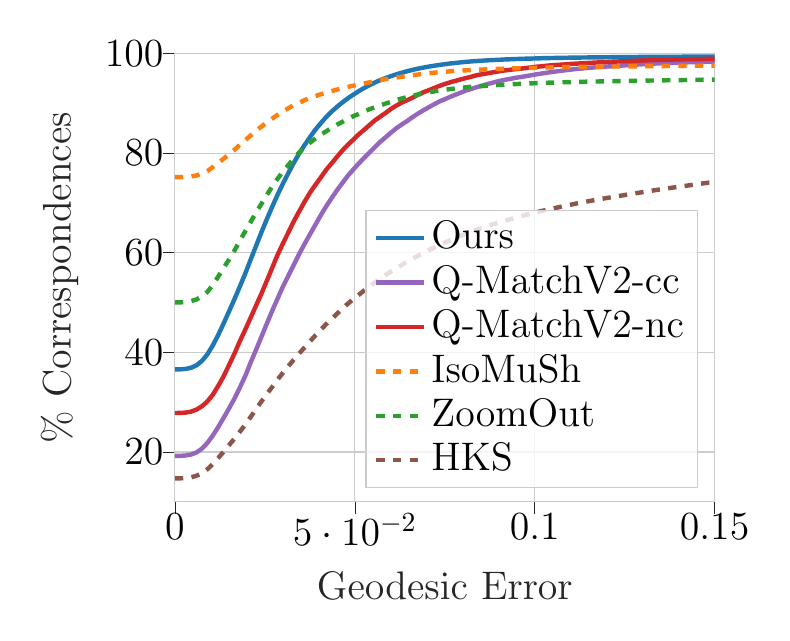
\begin{tikzpicture}

\definecolor{crimson2143940}{RGB}{214,39,40}
\definecolor{darkorange25512714}{RGB}{255,127,14}
\definecolor{darkslategray38}{RGB}{38,38,38}
\definecolor{forestgreen4416044}{RGB}{44,160,44}
\definecolor{lightgray204}{RGB}{204,204,204}
\definecolor{mediumpurple148103189}{RGB}{148,103,189}
\definecolor{sienna1408675}{RGB}{140,86,75}
\definecolor{steelblue31119180}{RGB}{31,119,180}

\Large
\begin{axis}[
axis line style={lightgray204},
legend cell align={left},
legend style={
  fill opacity=0.8,
  draw opacity=1,
  text opacity=1,
  at={(0.97,0.03)},
  anchor=south east,
  draw=lightgray204
},
xtick = {0,0.05,0.1,0.15},
ytick = {20,40,60,80,100},
xticklabel style={yshift= 5pt},
yticklabel style={xshift= 5pt},
tick align=outside,
tick pos=left,
x grid style={lightgray204},
xlabel=\textcolor{darkslategray38}{Geodesic Error},
xmajorgrids,
xmin=0, xmax=0.15,
xtick style={color=darkslategray38},
y grid style={lightgray204},
ylabel=\textcolor{darkslategray38}{\% Correspondences},
ymajorgrids,
ymin= 10, ymax=100,
ytick style={color=darkslategray38}
]
\addplot [ultra thick, steelblue31119180]
table {%
0 36.5777690650445
0.0015 36.5963509488959
0.003 36.6836089725311
0.0045 36.9177121946583
0.006 37.4088846117289
0.0075 38.2860429933783
0.009 39.6013964135222
0.0105 41.3659506384057
0.012 43.4547096283623
0.0135 45.7648710515477
0.015 48.1782308399075
0.0165 50.6061408928175
0.018 53.1527381744448
0.0195 55.750039603333
0.021 58.5415676583341
0.0225 61.2850370687197
0.024 64.0470249976238
0.0255 66.6662151886703
0.027 69.1682111966543
0.0285 71.6048419034946
0.03 73.8612378417768
0.0315 75.9606224059817
0.033 78.011619617907
0.0345 79.8930908025219
0.036 81.5825610683395
0.0375 83.1676646706587
0.039 84.681165446884
0.0405 85.974293476539
0.042 87.2300082374933
0.0435 88.3052585305579
0.045 89.2717818331591
0.0465 90.162955834363
0.048 90.9701826505719
0.0495 91.7000562367329
0.051 92.4020411557837
0.0525 93.0377736590312
0.054 93.6170238887305
0.0555 94.1523223394481
0.057 94.6379384088965
0.0585 95.0536941989038
0.06 95.4530225263758
0.0615 95.8099515255204
0.063 96.1319503849444
0.0645 96.4382782054938
0.066 96.7010304787251
0.0675 96.9536957830371
0.069 97.1668805246649
0.0705 97.3724614263536
0.072 97.5411082596711
0.0735 97.7063214840161
0.075 97.8479390425498
0.0765 98.0028316383107
0.078 98.1122873301017
0.0795 98.2322339448088
0.081 98.3330521496689
0.0825 98.4225319202864
0.084 98.4989584323417
0.0855 98.5666128061338
0.087 98.6392770015525
0.0885 98.6888603744891
0.09 98.7352754807845
0.0915 98.8000110889332
0.093 98.8420777492634
0.0945 98.8865918955739
0.096 98.9252328675981
0.0975 98.9616006083072
0.099 98.9866536767734
0.1005 99.013286918227
0.102 99.0519516522511
0.1035 99.0824660203403
0.105 99.1008182048601
0.1065 99.1194317713779
0.108 99.1413086525362
0.1095 99.1587460000634
0.111 99.1736328929443
0.1125 99.1899890694801
0.114 99.2010146373919
0.1155 99.2159292526059
0.117 99.2290379558344
0.1185 99.236162595444
0.12 99.2507405823274
0.1215 99.2604156765833
0.123 99.2727204321516
0.1245 99.2815321737477
0.126 99.2903953996768
0.1275 99.3003714792637
0.129 99.3091832208599
0.1305 99.3156979691411
0.132 99.3266680923867
0.1335 99.3321848366759
0.135 99.3382797896271
0.1365 99.3431034755885
0.138 99.3481489402148
0.1395 99.3512261191902
0.141 99.3581567024681
0.1425 99.363000190096
0.144 99.3655506447423
0.1455 99.3674912080601
0.147 99.3693961283781
0.1485 99.371336691696
0.15 99.371336691696
};
 \addlegendentry{Ours}

\addplot [ultra thick, mediumpurple148103189]
table {%
0 19.2065591040142
0.0015 19.2294023064981
0.003 19.3066367265469
0.0045 19.5028276779774
0.006 19.9180805056554
0.0075 20.6714903526281
0.009 21.8117099135063
0.0105 23.2729263694833
0.012 24.9774617431803
0.0135 26.8233532934132
0.015 28.7103016189842
0.0165 30.6700487913063
0.018 32.8595309381237
0.0195 35.1870980261699
0.021 37.8935185185185
0.0225 40.4378188068308
0.024 43.057163450876
0.0255 45.6969948990907
0.027 48.2943280106454
0.0285 50.7436238633843
0.03 53.1798902195609
0.0315 55.3515469061876
0.033 57.5362608117099
0.0345 59.7042304280328
0.036 61.7371645597693
0.0375 63.6530272787758
0.039 65.575543357729
0.0405 67.4892437347527
0.042 69.2753659347971
0.0435 70.9244011976048
0.045 72.4991128853404
0.0465 73.9672599245953
0.048 75.3996451541362
0.0495 76.6540252827678
0.051 77.8541805278332
0.0525 78.9901585717454
0.054 80.0780660900421
0.0555 81.1485362608117
0.057 82.2283488578399
0.0585 83.147122421823
0.06 84.0774839210468
0.0615 84.9687569305833
0.063 85.7261865158572
0.0645 86.4248170326015
0.066 87.2027334220448
0.0675 87.9280328232424
0.069 88.5690563317809
0.0705 89.1962186737636
0.072 89.7854291417166
0.0735 90.3724218230206
0.075 90.8174761587935
0.0765 91.2993457529386
0.078 91.7334220447993
0.0795 92.1617598137059
0.081 92.5918440895986
0.0825 92.9268130405855
0.084 93.2727323131515
0.0855 93.5833610556664
0.087 93.8990075404746
0.0885 94.178171434908
0.09 94.4513195830561
0.0915 94.7005156353959
0.093 94.8835107562652
0.0945 95.0979984475493
0.096 95.2684353515192
0.0975 95.4466345087603
0.099 95.6338434242626
0.1005 95.8247116877356
0.102 95.9929585273896
0.1035 96.1597360833888
0.105 96.3124029718341
0.1065 96.4520126413839
0.108 96.5875194056331
0.1095 96.7215014415613
0.111 96.8491905078731
0.1125 96.9556442670215
0.114 97.0588545131958
0.1155 97.1496728764693
0.117 97.2372477267687
0.1185 97.3203038367709
0.12 97.3845087602573
0.1215 97.4485196274119
0.123 97.5185462408516
0.1245 97.594921268574
0.126 97.6762585939232
0.1275 97.7438733643823
0.129 97.8021734309159
0.1305 97.8653526280772
0.132 97.9353792415169
0.1335 97.989326901752
0.135 98.0426646706587
0.1365 98.0825848303393
0.138 98.136199822577
0.1395 98.1593479707252
0.141 98.2050066533599
0.1425 98.2377744510978
0.144 98.2670215125305
0.1455 98.2967952982923
0.147 98.3332224440009
0.1485 98.3551785318253
0.15 98.3551785318253
};
 \addlegendentry{Q-MatchV2-cc }
\addplot [ultra thick, crimson2143940]
table {%
0 27.8302284320248
0.0015 27.8444777112442
0.003 27.9158904413396
0.0045 28.1185684187181
0.006 28.5204868041694
0.0075 29.1949157241073
0.009 30.1281049013085
0.0105 31.4784597471723
0.012 33.2379962297627
0.0135 35.1693834553116
0.015 37.4038589487691
0.0165 39.6816090042138
0.018 42.1834664005323
0.0195 44.48708139277
0.021 46.8973442004879
0.0225 49.3324184963407
0.024 51.724412286538
0.0255 54.3097139055223
0.027 56.9114548680417
0.0285 59.5429418939898
0.03 61.8442559325793
0.0315 64.0368429807052
0.033 66.2665779552007
0.0345 68.2605067642493
0.036 70.201042359725
0.0375 72.0177422931914
0.039 73.5849412286538
0.0405 75.075044355733
0.042 76.6185129740519
0.0435 77.9096529163894
0.045 79.2156797516079
0.0465 80.4944832557108
0.048 81.6387779995565
0.0495 82.6590984697272
0.051 83.7134342426258
0.0525 84.6318751386117
0.054 85.5865214016411
0.0555 86.5301341760922
0.057 87.2957972943003
0.0585 88.0463517409625
0.06 88.8542636948326
0.0615 89.526835218452
0.063 90.1345919272566
0.0645 90.5986083388778
0.066 91.1258593923264
0.0675 91.6982424040807
0.069 92.2055611000222
0.0705 92.6197050343757
0.072 93.0529773785762
0.0735 93.5000554446662
0.075 93.869538700377
0.0765 94.2226380572189
0.078 94.5210135284986
0.0795 94.8142603681526
0.081 95.0976935018851
0.0825 95.3621922821025
0.084 95.6688290086494
0.0855 95.8555666444888
0.087 96.0421656686626
0.0885 96.2426258593923
0.09 96.4196329563096
0.0915 96.5798403193613
0.093 96.7222776668885
0.0945 96.838711465957
0.096 96.9504324683966
0.0975 97.0782324240408
0.099 97.2185905965847
0.1005 97.3516023508539
0.102 97.4332446218674
0.1035 97.563872255489
0.105 97.6631182080284
0.1065 97.7260756265248
0.108 97.7968230206254
0.1095 97.8883067198936
0.111 97.9449157241073
0.1125 98.0114770459082
0.114 98.076790862719
0.1155 98.1336770902639
0.117 98.1902860944777
0.1185 98.2451485917055
0.12 98.2889498780218
0.1215 98.3524894655135
0.123 98.3939343535152
0.1245 98.4335772898647
0.126 98.4647649146152
0.1275 98.5215125304946
0.129 98.5670048791306
0.1305 98.6147427367487
0.132 98.6522233311156
0.1335 98.6856841871812
0.135 98.7146817476159
0.1365 98.7457584830339
0.138 98.7727600354846
0.1395 98.8091871811931
0.141 98.8303947660235
0.1425 98.8590596584608
0.144 98.8695941450432
0.1455 98.8855899312486
0.147 98.8979818141495
0.1485 98.9161953870037
0.15 98.9161953870037
};
 \addlegendentry{Q-MatchV2-nc }
\addplot [ultra thick, dashed,darkorange25512714]
table {%
0 75.1717213114754
0.0015 75.1848360655738
0.003 75.2213114754098
0.0045 75.3204918032787
0.006 75.5282786885246
0.0075 75.8803278688524
0.009 76.3905737704918
0.0105 77.1647540983607
0.012 78.0086065573771
0.0135 78.8729508196721
0.015 79.769262295082
0.0165 80.6327868852459
0.018 81.6598360655738
0.0195 82.5729508196721
0.021 83.5094262295082
0.0225 84.4545081967213
0.024 85.3159836065574
0.0255 86.1225409836065
0.027 86.9110655737705
0.0285 87.6680327868853
0.03 88.3774590163934
0.0315 88.9975409836065
0.033 89.6409836065574
0.0345 90.1131147540983
0.036 90.6225409836066
0.0375 91.0606557377049
0.039 91.4426229508197
0.0405 91.8102459016394
0.042 92.1102459016393
0.0435 92.4508196721312
0.045 92.7454918032787
0.0465 93.0008196721312
0.048 93.2770491803279
0.0495 93.5270491803279
0.051 93.7569672131148
0.0525 93.9795081967213
0.054 94.2045081967213
0.0555 94.4233606557378
0.057 94.6446721311475
0.0585 94.8434426229508
0.06 95.0127049180327
0.0615 95.177868852459
0.063 95.3303278688525
0.0645 95.4713114754098
0.066 95.6377049180327
0.0675 95.7803278688524
0.069 95.9151639344262
0.0705 96.0459016393443
0.072 96.1565573770492
0.0735 96.2446721311475
0.075 96.3487704918033
0.0765 96.4213114754099
0.078 96.5147540983607
0.0795 96.5790983606558
0.081 96.630737704918
0.0825 96.6889344262296
0.084 96.7331967213115
0.0855 96.7840163934427
0.087 96.8393442622951
0.0885 96.8704918032787
0.09 96.9204918032787
0.0915 96.9545081967214
0.093 96.991393442623
0.0945 97.0241803278689
0.096 97.0520491803279
0.0975 97.0852459016394
0.099 97.1176229508197
0.1005 97.15
0.102 97.1700819672131
0.1035 97.1934426229509
0.105 97.2094262295083
0.1065 97.2303278688525
0.108 97.2565573770492
0.1095 97.2733606557378
0.111 97.2868852459017
0.1125 97.2991803278689
0.114 97.316393442623
0.1155 97.3315573770492
0.117 97.3450819672132
0.1185 97.3573770491804
0.12 97.3680327868853
0.1215 97.3852459016394
0.123 97.4012295081968
0.1245 97.4114754098361
0.126 97.419262295082
0.1275 97.4237704918033
0.129 97.4323770491804
0.1305 97.4491803278689
0.132 97.4668032786886
0.1335 97.4741803278689
0.135 97.4819672131148
0.1365 97.488524590164
0.138 97.497131147541
0.1395 97.5081967213115
0.141 97.5176229508197
0.1425 97.5311475409836
0.144 97.5368852459017
0.1455 97.5475409836066
0.147 97.5569672131147
0.1485 97.5647540983607
0.15 97.5647540983607
};
 \addlegendentry{IsoMuSh }
\addplot [ultra thick, dashed, forestgreen4416044]
table {%
0 50.0203703703704
0.0015 50.0412037037037
0.003 50.1050925925926
0.0045 50.300462962963
0.006 50.625462962963
0.0075 51.2467592592593
0.009 52.1282407407407
0.0105 53.512037037037
0.012 55.1847222222222
0.0135 56.8986111111111
0.015 58.5921296296296
0.0165 60.3773148148148
0.018 62.3430555555556
0.0195 64.2759259259259
0.021 66.1138888888889
0.0225 68.0226851851852
0.024 69.7754629629629
0.0255 71.5365740740741
0.027 73.2675925925926
0.0285 74.8259259259259
0.03 76.2851851851852
0.0315 77.5912037037037
0.033 78.9013888888889
0.0345 80.0898148148148
0.036 81.1685185185185
0.0375 82.0888888888889
0.039 82.8958333333334
0.0405 83.6787037037037
0.042 84.3606481481482
0.0435 85.0481481481482
0.045 85.7
0.0465 86.2736111111111
0.048 86.8407407407407
0.0495 87.4037037037037
0.051 87.8379629629629
0.0525 88.3458333333333
0.054 88.7916666666666
0.0555 89.2018518518518
0.057 89.5712962962963
0.0585 89.9379629629629
0.06 90.287037037037
0.0615 90.637037037037
0.063 90.9587962962963
0.0645 91.2462962962964
0.066 91.5162037037037
0.0675 91.7634259259259
0.069 91.9930555555556
0.0705 92.1842592592593
0.072 92.3916666666667
0.0735 92.5824074074074
0.075 92.7305555555555
0.0765 92.8587962962963
0.078 92.9967592592593
0.0795 93.1250000000001
0.081 93.2199074074074
0.0825 93.3185185185185
0.084 93.3879629629629
0.0855 93.4763888888888
0.087 93.5560185185185
0.0885 93.625
0.09 93.6875
0.0915 93.7486111111111
0.093 93.8087962962963
0.0945 93.8615740740741
0.096 93.9055555555556
0.0975 93.9648148148148
0.099 94.0087962962963
0.1005 94.0495370370371
0.102 94.0921296296296
0.1035 94.1319444444444
0.105 94.1675925925926
0.1065 94.1944444444445
0.108 94.2324074074075
0.1095 94.2643518518519
0.111 94.2921296296297
0.1125 94.3115740740741
0.114 94.3356481481482
0.1155 94.3597222222223
0.117 94.3782407407408
0.1185 94.3981481481483
0.12 94.4203703703704
0.1215 94.4342592592593
0.123 94.4537037037038
0.1245 94.4717592592593
0.126 94.500462962963
0.1275 94.5199074074075
0.129 94.5347222222223
0.1305 94.5532407407408
0.132 94.575462962963
0.1335 94.5916666666667
0.135 94.6106481481482
0.1365 94.625462962963
0.138 94.6398148148149
0.1395 94.6527777777778
0.141 94.6694444444445
0.1425 94.6925925925927
0.144 94.7087962962964
0.1455 94.7296296296297
0.147 94.7435185185186
0.1485 94.7569444444445
0.15 94.7569444444445
};
 \addlegendentry{ZoomOut }

\addplot [ultra thick, dashed, sienna1408675]
table {%
0 14.7003215790641
0.0015 14.7177312042581
0.003 14.7653146088775
0.0045 14.9225754839527
0.006 15.2381902860945
0.0075 15.7476515223521
0.009 16.5300510090929
0.0105 17.592295567595
0.012 18.7731125051484
0.0135 20.0321420650762
0.015 21.3487984348763
0.0165 22.6572410734087
0.018 24.021872920825
0.0195 25.462622374299
0.021 26.9911446947375
0.0225 28.5729453790831
0.024 30.10583198682
0.0255 31.6135150334252
0.027 33.0302054620917
0.0285 34.5102414219181
0.03 35.8817008839464
0.0315 37.2104402306498
0.033 38.5074414662738
0.0345 39.7634057282261
0.036 40.9564402940151
0.0375 42.1758467192599
0.039 43.3739029876754
0.0405 44.5212075848303
0.042 45.6407660868739
0.0435 46.6848921205209
0.045 47.7170341855971
0.0465 48.7497623800019
0.048 49.744669391376
0.0495 50.6341602509267
0.051 51.5000198016665
0.0525 52.3723663783544
0.054 53.2258459271932
0.0555 54.0045306212971
0.057 54.7779520324431
0.0585 55.5109701232456
0.06 56.1934107974527
0.0615 56.8701644330387
0.063 57.5383954313595
0.0645 58.1772328359155
0.066 58.7896033330165
0.0675 59.3724693470202
0.069 59.9479651807496
0.0705 60.5078612616038
0.072 61.0340667870608
0.0735 61.5364152647087
0.075 62.0323836454076
0.0765 62.5030415359757
0.078 62.973663783544
0.0795 63.4149360010138
0.081 63.8453846275703
0.0825 64.2442337547128
0.084 64.6715655989608
0.0855 65.0280629217755
0.087 65.3833166999335
0.0885 65.7259092925261
0.09 66.0562486138834
0.0915 66.3756732566613
0.093 66.7035730127047
0.0945 66.9865863511073
0.096 67.2997497069353
0.0975 67.5869966416374
0.099 67.8644853150841
0.1005 68.1304335772899
0.102 68.3978273611507
0.1035 68.6452333428381
0.105 68.8697010740424
0.1065 69.116045686405
0.108 69.3493608022051
0.1095 69.5627237588315
0.111 69.8074921585401
0.1125 70.0179680321896
0.114 70.2320319678104
0.1155 70.4181240693216
0.117 70.6218317333587
0.1185 70.8050407122264
0.12 70.9926654627253
0.1215 71.1703220543041
0.123 71.35707949181
0.1245 71.5251639577987
0.126 71.7105511199823
0.1275 71.8865720939074
0.129 72.0521021449165
0.1305 72.2246815892025
0.132 72.4001243544657
0.1335 72.5688424737826
0.135 72.7278062921776
0.1365 72.8904571808763
0.138 73.0399043183474
0.1395 73.2029433197098
0.141 73.3425727909261
0.1425 73.4937149510503
0.144 73.6461085764978
0.1455 73.8056783258879
0.147 73.9477909260843
0.1485 74.08875106929
0.15 74.08875106929
};
\addlegendentry{HKS}
\end{axis}

\end{tikzpicture}
}
      \caption{SMAL \cite{Zuffi:CVPR:2017}}
      \label{fig:SMALquant}
    
    \end{subfigure}
    \vspace{-1em}
    \caption{
    Quantitative results on all three datasets. %
    For each dataset, we match all shapes within a class and then plot the average PCK curve across classes. 
    We plot classical methods with dashed lines as they are only for reference. 
    HKS is our initialisation (see Sec.~\ref{sec:n_shapes}). 
    }
    \label{fig:FAUST_TOSCA_SMAL}
    \vspace{-1em}
\end{figure*}




\noindent\textbf{FAUST.} 
We outperform both quantum and classical prior work, as Fig.~\ref{fig:FAUSTquant} and Tab.~\ref{Table:FAUST_TOSCA_SMAL} show. 
Because we downsample FAUST more, IsoMuSh's results are better in our experiments than what Gao \textit{et al.}~\cite{Gao2021} report.


\noindent\textbf{Matching $\mathbf{100}$ Shapes.} 
Next, we demonstrate that, unlike IsoMuSh and ZoomOut, our approach can scale to matching all 100 shapes of FAUST. %
Fig.~\ref{fig:teaser} contains qualitative results.
Tab.~\ref{tab:runtime} compares the runtime of our method (using SA) to others. 
Only ours and Q-MatchV2-cc scale well to $100$ shapes while ZoomOut and IsoMuSh cannot. 

\begin{table}[h]
    \centering
    \resizebox{\linewidth}{!}{
    \begin{tabular}{|c|ccccc|}
    \hline
    \# Shapes       & Ours & Q-MatchV2-cc & Q-MatchV2-nc         & IsoMuSh & ZoomOut    \\
    \hline\hline
    10              & 97   & 16           & 81                   & $(4+)0.3$ & \textbf{4} \\
    100             & 1137 & \textbf{175} & ${\sim}8000^\dagger$ & OOM     & OOM        \\
    \hline
    \end{tabular}
    }
    \caption{Runtime (in \textit{min}) for FAUST. IsoMuSh uses ZoomOut for initialisation. 
    ``OOM''  (out of memory): memory requirements are infeasible. ``$^\dagger$'' denotes an estimate. %
    }
    \label{tab:runtime}
\end{table}


    


\noindent\textbf{TOSCA.} 
Fig.~\ref{fig:TOSCAquant} and Tab.~\ref{Table:FAUST_TOSCA_SMAL} show that our method achieves state-of-the-art results.
While IsoMuSh's PCK curve starts higher (better), the AUC in Tab.~\ref{Table:FAUST_TOSCA_SMAL} suggests that our method performs better overall. 
Fig.~\ref{fig:tosca_qualitative} has qualitative examples. 


\noindent\textbf{SMAL.} 
Our CCuantuMM outperforms the quantum baselines, both in terms of PCK (Fig.~\ref{fig:SMALquant}) and AUC (Tab.~\ref{Table:FAUST_TOSCA_SMAL}). 
At the same time, it achieves performance on par with ZoomOut and below IsoMuSh. 
SMAL is considered the most difficult of the three datasets due to the challenging non-isometric deformations of its shapes. 
All methods thus show worse performance compared to FAUST and TOSCA. 

    

    



\subsection{Ablation Studies} 
We perform an ablation study on FAUST to analyse how different components of our method affect the quality of the matchings. 
We refer to the supplement for more ablations. 

\begin{figure}%
    \resizebox{0.49\linewidth}{!}{
    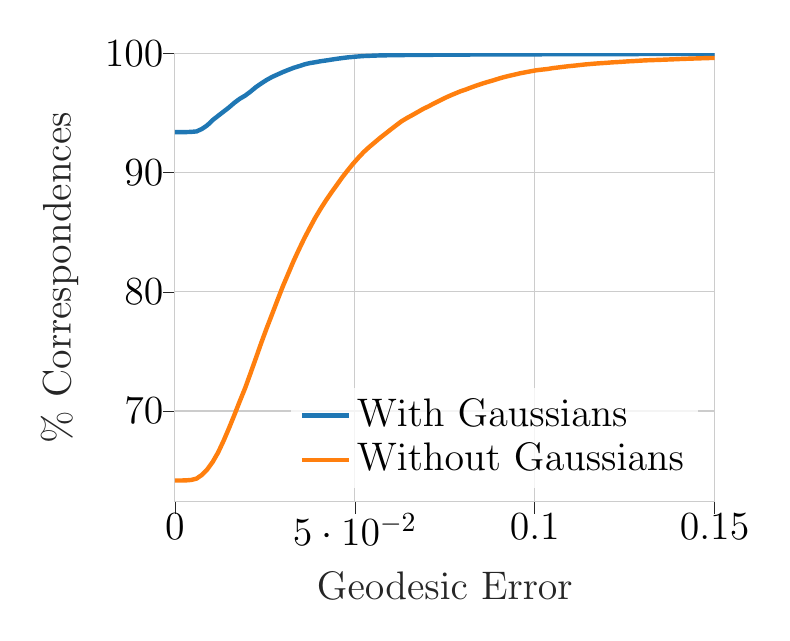
\begin{tikzpicture}

\definecolor{darkorange25512714}{RGB}{255,127,14}
\definecolor{darkslategray38}{RGB}{38,38,38}
\definecolor{lightgray204}{RGB}{204,204,204}
\definecolor{steelblue31119180}{RGB}{31,119,180}

\Large 
\begin{axis}[
axis line style={lightgray204},
legend cell align={left},
legend style={
  fill opacity=0.8,
  draw opacity=1,
  text opacity=1,
  at={(0.97,0.03)},
  anchor=south east,
  draw=none
},
tick align=outside,
tick pos=left,
x grid style={lightgray204},
xlabel=\textcolor{darkslategray38}{Geodesic Error},
xmajorgrids,
xmin=0, xmax=0.15,
xtick style={color=darkslategray38},
xtick ={0,0.05,0.1,0.15},
y grid style={lightgray204},
ylabel=\textcolor{darkslategray38}{\% Correspondences},
ymin=62.3818061088978, ymax=100,
ymajorgrids,
xticklabel style={yshift= 5pt},
yticklabel style={xshift= 5pt},
ytick style={color=darkslategray38}
]
\addplot [ultra thick, steelblue31119180]
table {%
0 93.4019477644976
0.0015 93.4021691013723
0.003 93.4074811863656
0.0045 93.4229747675963
0.006 93.4645861000443
0.0075 93.6702080566622
0.009 93.9803010181496
0.0105 94.4156706507304
0.012 94.7726870296591
0.0135 95.1188579017264
0.015 95.4712262062859
0.0165 95.8612217795485
0.018 96.199203187251
0.0195 96.4645861000443
0.021 96.8025675077468
0.0225 97.1790615316512
0.024 97.4922532093847
0.0255 97.7833111996458
0.027 98.0336432049579
0.0285 98.2386011509517
0.03 98.4420097388225
0.0315 98.6250553342187
0.033 98.7990261177512
0.0345 98.9389110225763
0.036 99.0894200973882
0.0375 99.1963258078796
0.039 99.2682602921646
0.0405 99.3530323151836
0.042 99.4156706507303
0.0435 99.4873837981407
0.045 99.5559982293049
0.0465 99.6177512173528
0.048 99.6757414785303
0.0495 99.7153607791058
0.051 99.7563081009296
0.0525 99.7886232846392
0.054 99.8065515714918
0.0555 99.8247011952191
0.057 99.839973439575
0.0585 99.847941567065
0.06 99.8601150951748
0.0615 99.8634351482957
0.063 99.8691899070385
0.0645 99.8747233289066
0.066 99.881584772023
0.0675 99.8851261620185
0.069 99.8860115095174
0.0705 99.8906595838866
0.072 99.893536963258
0.0735 99.8968570163789
0.075 99.9026117751217
0.0765 99.9052678176184
0.078 99.9061531651173
0.0795 99.9065958388667
0.081 99.9096945551128
0.0825 99.9163346613546
0.084 99.9196547144754
0.0855 99.9225320938468
0.087 99.9260734838424
0.0885 99.9267374944666
0.09 99.9280655157149
0.0915 99.9285081894643
0.093 99.9285081894643
0.0945 99.9293935369632
0.096 99.9318282425852
0.0975 99.9322709163346
0.099 99.9324922532093
0.1005 99.9329349269588
0.102 99.935148295706
0.1035 99.9393536963258
0.105 99.9393536963258
0.1065 99.9424524125719
0.108 99.9424524125719
0.1095 99.9431164231961
0.111 99.9446657813191
0.1125 99.945551128818
0.114 99.9459938025675
0.1155 99.9464364763169
0.117 99.9475431606906
0.1185 99.9510845506861
0.12 99.951969898185
0.1215 99.9528552456839
0.123 99.9532979194334
0.1245 99.954404603807
0.126 99.9552899513059
0.1275 99.95595396193
0.129 99.9561752988048
0.1305 99.9572819831784
0.132 99.9581673306773
0.1335 99.9586100044267
0.135 99.9586100044267
0.1365 99.9586100044267
0.138 99.9586100044267
0.1395 99.9588313413014
0.141 99.9590526781762
0.1425 99.9610447100487
0.144 99.9612660469234
0.1455 99.9612660469234
0.147 99.9612660469234
0.1485 99.9614873837981
0.15 99.9614873837981
};
\addlegendentry{With Gaussians}
\addplot [ultra thick, darkorange25512714]
table {%
0 64.1713147410359
0.0015 64.17197875166
0.003 64.1812749003984
0.0045 64.2184594953519
0.006 64.3326693227092
0.0075 64.6423196104471
0.009 65.1117751217353
0.0105 65.736830455954
0.012 66.5245683930943
0.0135 67.4889331562638
0.015 68.5444887118194
0.0165 69.6580345285525
0.018 70.8089862771138
0.0195 71.9194333776007
0.021 73.1677733510403
0.0225 74.4402390438247
0.024 75.7297476759628
0.0255 76.9541832669323
0.027 78.1250553342187
0.0285 79.3076582558654
0.03 80.4721115537849
0.0315 81.5360779105799
0.033 82.6022576361222
0.0345 83.5792386011509
0.036 84.5179282868526
0.0375 85.3802567507747
0.039 86.2202301903497
0.0405 86.9760956175299
0.042 87.6834882691456
0.0435 88.3430721558212
0.045 88.9725542275343
0.0465 89.6091190792386
0.048 90.1892430278884
0.0495 90.7476759628154
0.051 91.259185480301
0.0525 91.7392651615759
0.054 92.1549358123063
0.0555 92.5336432049579
0.057 92.9183266932271
0.0585 93.2718016821602
0.06 93.6288180610889
0.0615 93.9760956175299
0.063 94.3173970783533
0.0645 94.5900841080124
0.066 94.8373173970784
0.0675 95.0925188136343
0.069 95.3541389995573
0.0705 95.5672864099159
0.072 95.8123063302346
0.0735 96.0345285524568
0.075 96.2636122177955
0.0765 96.4679061531651
0.078 96.6586985391766
0.0795 96.8459495351925
0.081 96.9962372731297
0.0825 97.1699867197875
0.084 97.3324479858344
0.0855 97.4811863656485
0.087 97.6206285967242
0.0885 97.7496679946879
0.09 97.893536963258
0.0915 98.0227976980965
0.093 98.1336874723328
0.0945 98.235945108455
0.096 98.3426294820717
0.0975 98.4289508632138
0.099 98.5150509074811
0.1005 98.5962815405046
0.102 98.6496237273129
0.1035 98.6978751660026
0.105 98.773572377158
0.1065 98.827135900841
0.108 98.883134130146
0.1095 98.939132359451
0.111 98.9820717131473
0.1125 99.0325365205843
0.114 99.082337317397
0.1155 99.1206285967241
0.117 99.1584772023018
0.1185 99.1901283753873
0.12 99.2186808322266
0.1215 99.2569721115537
0.123 99.2813191677733
0.1245 99.3116423196104
0.126 99.3428508189463
0.1275 99.3658698539176
0.129 99.3930942895086
0.1305 99.4218680832226
0.132 99.4402390438246
0.1335 99.4555112881805
0.135 99.4707835325365
0.1365 99.4900398406374
0.138 99.5070827799911
0.1395 99.5261177512173
0.141 99.5462594068171
0.1425 99.5610889774236
0.144 99.5770252324037
0.1455 99.5914121292606
0.147 99.6060203629924
0.1485 99.6210712704736
0.15 99.6210712704736
};
\addlegendentry{Without Gaussians}
\end{axis}

\end{tikzpicture}

    }
    \resizebox{0.49\linewidth}{!}{
    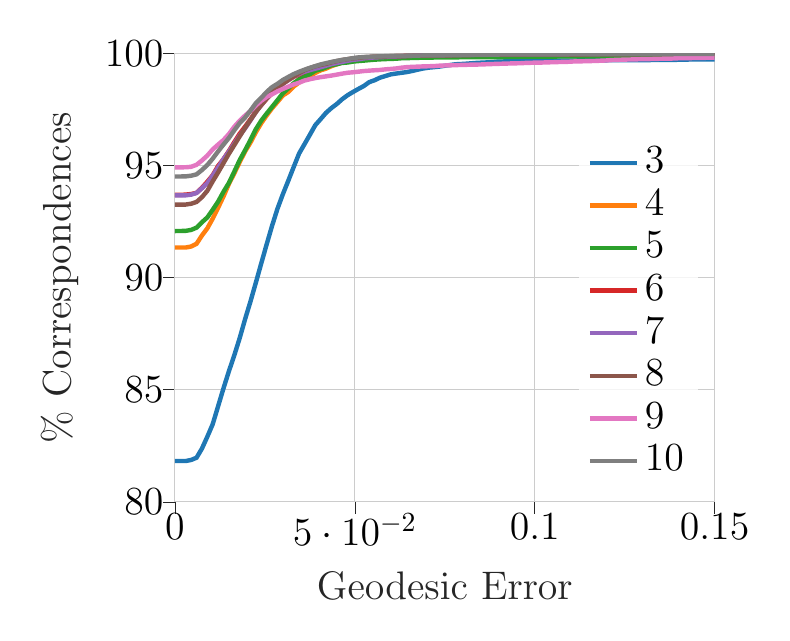
\begin{tikzpicture}

\definecolor{crimson2143940}{RGB}{214,39,40}
\definecolor{darkorange25512714}{RGB}{255,127,14}
\definecolor{darkslategray38}{RGB}{38,38,38}
\definecolor{forestgreen4416044}{RGB}{44,160,44}
\definecolor{gray127}{RGB}{127,127,127}
\definecolor{lightgray204}{RGB}{204,204,204}
\definecolor{mediumpurple148103189}{RGB}{148,103,189}
\definecolor{orchid227119194}{RGB}{227,119,194}
\definecolor{sienna1408675}{RGB}{140,86,75}
\definecolor{steelblue31119180}{RGB}{31,119,180}

\Large 
\begin{axis}[
axis line style={lightgray204},
legend cell align={left},
legend style={
  fill opacity=0.8,
  draw opacity=1,
  text opacity=1,
  at={(0.97,0.03)},
  anchor=south east,
  draw=none
},
tick align=outside,
tick pos=left,
x grid style={lightgray204},
xlabel=\textcolor{darkslategray38}{Geodesic Error},
xmin=0, xmax=0.15,
xtick style={color=darkslategray38},
xmajorgrids,
xtick ={0,0.05,0.1,0.15},
xticklabel style={yshift= 5pt},
yticklabel style={xshift= 5pt},
y grid style={lightgray204},
ylabel=\textcolor{darkslategray38}{\% Correspondences},
ymin=80, ymax=100,
ymajorgrids,
ytick style={color=darkslategray38}
]
\addplot [ultra thick, steelblue31119180]
table {%
0 81.8208646893906
0.0015 81.8208646893906
0.003 81.8208646893906
0.0045 81.8688210122473
0.006 81.9684226058728
0.0075 82.3742068761989
0.009 82.9054153755349
0.0105 83.4661354581673
0.012 84.2666371550834
0.0135 85.0671388519994
0.015 85.8270621218828
0.0165 86.5390290689095
0.018 87.3063302346171
0.0195 88.1510993064778
0.021 88.9405341596577
0.0225 89.7816142836063
0.024 90.6448280950273
0.0255 91.489597166888
0.027 92.3159214991884
0.0285 93.0758447690719
0.03 93.7250996015936
0.0315 94.3227091633466
0.033 94.9350745167478
0.0345 95.5363730264129
0.036 95.9532241404751
0.0375 96.3737642024495
0.039 96.8016821602479
0.0405 97.07466430574
0.042 97.3550243470562
0.0435 97.5689833259554
0.045 97.7497417736462
0.0465 97.9637007525454
0.048 98.140770252324
0.0495 98.2846392208942
0.051 98.4211302936402
0.0525 98.5502434705622
0.054 98.7236240224288
0.0555 98.8084698244061
0.057 98.9228272096798
0.0585 98.9966061679209
0.06 99.070385126162
0.0615 99.1072746052826
0.063 99.1404751364911
0.0645 99.1736756676996
0.066 99.2216319905563
0.0675 99.2806551571492
0.069 99.332300427918
0.0705 99.3691899070385
0.072 99.3913235945109
0.0735 99.4171462298952
0.075 99.4540357090158
0.0765 99.4872362402243
0.078 99.5204367714328
0.0795 99.531503615169
0.081 99.5462594068172
0.0825 99.5647041463775
0.084 99.5831488859377
0.0855 99.5942157296739
0.087 99.6052825734101
0.0885 99.6200383650583
0.09 99.6421720525306
0.0915 99.6458610004427
0.093 99.6458610004427
0.0945 99.6495499483547
0.096 99.6532388962668
0.0975 99.6606167920909
0.099 99.664305740003
0.1005 99.6716836358271
0.102 99.6753725837391
0.1035 99.6753725837391
0.105 99.6790615316512
0.1065 99.6790615316512
0.108 99.6827504795633
0.1095 99.6827504795633
0.111 99.6864394274753
0.1125 99.6938173232994
0.114 99.6938173232994
0.1155 99.6938173232994
0.117 99.6975062712115
0.1185 99.6975062712115
0.12 99.6975062712115
0.1215 99.7011952191235
0.123 99.7011952191235
0.1245 99.7011952191235
0.126 99.7048841670356
0.1275 99.7048841670356
0.129 99.7048841670356
0.1305 99.7048841670356
0.132 99.7085731149476
0.1335 99.7122620628597
0.135 99.7122620628597
0.1365 99.7196399586838
0.138 99.7196399586838
0.1395 99.7196399586838
0.141 99.73070680242
0.1425 99.73070680242
0.144 99.734395750332
0.1455 99.734395750332
0.147 99.7380846982441
0.1485 99.7380846982441
0.15 99.7380846982441
};
\addlegendentry{3}
\addplot [ultra thick, darkorange25512714]
table {%
0 91.3457281983178
0.0015 91.3457281983178
0.003 91.3457281983178
0.0045 91.3899955732625
0.006 91.5098863804043
0.0075 91.8806256455659
0.009 92.2015641139147
0.0105 92.6368599675372
0.012 93.1201121440165
0.0135 93.6273424819242
0.015 94.1825291426885
0.0165 94.6584034233437
0.018 95.1545669175151
0.0195 95.6341301460823
0.021 96.0288475726723
0.0225 96.4918105356352
0.024 96.8939058580493
0.0255 97.2388224878265
0.027 97.5597609561753
0.0285 97.8401209974915
0.03 98.1278589346318
0.0315 98.2846392208942
0.033 98.5281097830899
0.0345 98.7051792828685
0.036 98.8840932566032
0.0375 98.9984506418769
0.039 99.1312527667109
0.0405 99.2492990998967
0.042 99.3267670060499
0.0435 99.4355909694555
0.045 99.5204367714328
0.0465 99.599749151542
0.048 99.667994687915
0.0495 99.7067286409916
0.051 99.7436181201121
0.0525 99.7546849638483
0.054 99.7675962815405
0.0555 99.7786631252767
0.057 99.7915744429689
0.0585 99.800796812749
0.06 99.8081747085731
0.0615 99.8081747085731
0.063 99.8118636564852
0.0645 99.8247749741774
0.066 99.8284639220894
0.0675 99.8284639220894
0.069 99.8358418179135
0.0705 99.8505976095618
0.072 99.8727312970341
0.0735 99.8782647189022
0.075 99.8856426147263
0.0765 99.8911760365944
0.078 99.8985539324185
0.0795 99.9022428803305
0.081 99.9059318282426
0.0825 99.9059318282426
0.084 99.9096207761546
0.0855 99.9096207761546
0.087 99.9096207761546
0.0885 99.9096207761546
0.09 99.9133097240667
0.0915 99.9133097240667
0.093 99.9133097240667
0.0945 99.9151541980227
0.096 99.9206876198908
0.0975 99.9206876198908
0.099 99.9206876198908
0.1005 99.9262210417589
0.102 99.9262210417589
0.1035 99.9262210417589
0.105 99.9262210417589
0.1065 99.9262210417589
0.108 99.9262210417589
0.1095 99.9262210417589
0.111 99.9280655157149
0.1125 99.9280655157149
0.114 99.9280655157149
0.1155 99.9280655157149
0.117 99.929909989671
0.1185 99.929909989671
0.12 99.929909989671
0.1215 99.933598937583
0.123 99.933598937583
0.1245 99.935443411539
0.126 99.9428213073631
0.1275 99.9428213073631
0.129 99.9428213073631
0.1305 99.9428213073631
0.132 99.9446657813192
0.1335 99.9465102552752
0.135 99.9465102552752
0.1365 99.9501992031873
0.138 99.9501992031873
0.1395 99.9538881510993
0.141 99.9538881510993
0.1425 99.9557326250553
0.144 99.9594215729674
0.1455 99.9594215729674
0.147 99.9594215729674
0.1485 99.9631105208794
0.15 99.9631105208794
};
\addlegendentry{4}
\addplot [ultra thick, forestgreen4416044]
table {%
0 92.0805666223993
0.0015 92.0816733067729
0.003 92.0894200973882
0.0045 92.130367419212
0.006 92.2321823815848
0.0075 92.471226206286
0.009 92.6870296591412
0.0105 93.031208499336
0.012 93.3908809207614
0.0135 93.8335546702081
0.015 94.2275343072156
0.0165 94.7310756972111
0.018 95.2456839309429
0.0195 95.6850376272687
0.021 96.1454183266932
0.0225 96.6257193448428
0.024 97.0075254537406
0.0255 97.3218238158477
0.027 97.6195219123506
0.0285 97.9183266932271
0.03 98.2281983178398
0.0315 98.4395750332006
0.033 98.6752988047809
0.0345 98.8512616201859
0.036 98.9796370075255
0.0375 99.0770252324037
0.039 99.2308543603364
0.0405 99.2994687915007
0.042 99.3813634351483
0.0435 99.4743249225321
0.045 99.5230190349712
0.0465 99.5805666223993
0.048 99.5993802567508
0.0495 99.6403275785746
0.051 99.6635679504206
0.0525 99.6834882691457
0.054 99.7045152722444
0.0555 99.7255422753431
0.057 99.7399291722001
0.0585 99.7521027003099
0.06 99.7598494909252
0.0615 99.7687029659141
0.063 99.7897299690129
0.0645 99.7930500221337
0.066 99.8030101814962
0.0675 99.8074369189907
0.069 99.815183709606
0.0705 99.8196104471005
0.072 99.8207171314741
0.0735 99.8229305002213
0.075 99.8251438689686
0.0765 99.8295706064631
0.078 99.8295706064631
0.0795 99.8328906595839
0.081 99.8328906595839
0.0825 99.8328906595839
0.084 99.8328906595839
0.0855 99.8328906595839
0.087 99.8362107127047
0.0885 99.838424081452
0.09 99.838424081452
0.0915 99.8428508189464
0.093 99.8461708720673
0.0945 99.8472775564409
0.096 99.8550243470562
0.0975 99.8561310314298
0.099 99.8561310314298
0.1005 99.8561310314298
0.102 99.8572377158035
0.1035 99.8594510845507
0.105 99.8616644532979
0.1065 99.8660911907924
0.108 99.8694112439132
0.1095 99.8694112439132
0.111 99.8694112439132
0.1125 99.8694112439132
0.114 99.8694112439132
0.1155 99.8694112439132
0.117 99.8694112439132
0.1185 99.8694112439132
0.12 99.8705179282869
0.1215 99.8705179282869
0.123 99.8705179282869
0.1245 99.8705179282869
0.126 99.8705179282869
0.1275 99.8705179282869
0.129 99.8705179282869
0.1305 99.8705179282869
0.132 99.8716246126605
0.1335 99.8716246126605
0.135 99.8716246126605
0.1365 99.8716246126605
0.138 99.8716246126605
0.1395 99.8716246126605
0.141 99.8716246126605
0.1425 99.8716246126605
0.144 99.8716246126605
0.1455 99.8716246126605
0.147 99.8716246126605
0.1485 99.8716246126605
0.15 99.8716246126605
};
\addlegendentry{5}
\addplot [ultra thick, crimson2143940]
table {%
0 93.6918990703851
0.0015 93.6918990703851
0.003 93.7066548620334
0.0045 93.7302641286705
0.006 93.7848605577689
0.0075 94.0113619595691
0.009 94.2813929467316
0.0105 94.5720820422016
0.012 94.9867197875166
0.0135 95.2914268850524
0.015 95.6529437804338
0.0165 96.0476612070238
0.018 96.4246716836358
0.0195 96.7374944665781
0.021 97.070975357828
0.0225 97.435443411539
0.024 97.6951453445477
0.0255 97.979194333776
0.027 98.2248782647189
0.0285 98.4491662977719
0.03 98.6498450641877
0.0315 98.8128965619006
0.033 98.958978899218
0.0345 99.0630072303379
0.036 99.1899070385126
0.0375 99.2725394717427
0.039 99.3500073778958
0.0405 99.4171462298953
0.042 99.485022871477
0.0435 99.5654419359599
0.045 99.6111848900694
0.0465 99.6716836358271
0.048 99.718164379519
0.0495 99.7616939648812
0.051 99.7919433377601
0.0525 99.8199793418917
0.054 99.8339973439575
0.0555 99.8443263981113
0.057 99.8539176626826
0.0585 99.8583444001771
0.06 99.8701490334957
0.0615 99.8804780876494
0.063 99.8871181938911
0.0645 99.8974472480449
0.066 99.9018739855393
0.0675 99.9092518813634
0.069 99.9181053563524
0.0705 99.9225320938468
0.072 99.9328611480006
0.0735 99.9350745167478
0.075 99.9424524125719
0.0765 99.9431902021543
0.078 99.9431902021543
0.0795 99.9439279917368
0.081 99.9476169396488
0.0825 99.9483547292312
0.084 99.949830308396
0.0855 99.9513058875609
0.087 99.9513058875609
0.0885 99.9542570458905
0.09 99.9549948354729
0.0915 99.9564704146377
0.093 99.9645861000443
0.0945 99.9645861000443
0.096 99.9660616792091
0.0975 99.9667994687915
0.099 99.9704884167035
0.1005 99.9704884167035
0.102 99.9727017854508
0.1035 99.9727017854508
0.105 99.9734395750332
0.1065 99.9741773646156
0.108 99.9741773646156
0.1095 99.9741773646156
0.111 99.974915154198
0.1125 99.9756529437804
0.114 99.9786041021101
0.1155 99.9786041021101
0.117 99.9786041021101
0.1185 99.9786041021101
0.12 99.9800796812749
0.1215 99.9800796812749
0.123 99.9800796812749
0.1245 99.9800796812749
0.126 99.9800796812749
0.1275 99.9800796812749
0.129 99.9800796812749
0.1305 99.9815552604397
0.132 99.9815552604397
0.1335 99.9815552604397
0.135 99.9815552604397
0.1365 99.9822930500221
0.138 99.9822930500221
0.1395 99.9830308396046
0.141 99.9830308396046
0.1425 99.983768629187
0.144 99.983768629187
0.1455 99.983768629187
0.147 99.983768629187
0.1485 99.983768629187
0.15 99.983768629187
};
\addlegendentry{6}
\addplot [ultra thick, mediumpurple148103189]
table {%
0 93.672927338266
0.0015 93.672927338266
0.003 93.6734543308249
0.0045 93.7045468917979
0.006 93.7793798351567
0.0075 93.9912308438205
0.009 94.2167836590148
0.0105 94.5545858892472
0.012 94.9203187250996
0.0135 95.2892135163052
0.015 95.6206918358313
0.0165 95.981154746095
0.018 96.3416176563587
0.0195 96.6615021395898
0.021 97.019857079618
0.0225 97.3956027740888
0.024 97.7086363540547
0.0255 98.0021712093425
0.027 98.2456417715382
0.0285 98.441683003436
0.03 98.6508990493055
0.0315 98.8089968169649
0.033 98.9818503762727
0.0345 99.0909378359578
0.036 99.1937013849364
0.0375 99.257994477118
0.039 99.3212335841818
0.0405 99.3892156242754
0.042 99.4566706718101
0.0435 99.5278146672569
0.045 99.5789329454668
0.0465 99.6258352832058
0.048 99.6764265688569
0.0495 99.7175319884483
0.051 99.7433546238327
0.0525 99.7834060583065
0.054 99.8044857606611
0.0555 99.8260924555745
0.057 99.8345243365164
0.0585 99.8461181728114
0.06 99.8619279495774
0.0615 99.8645629123717
0.063 99.8798456965788
0.0645 99.8888045700795
0.066 99.8993444212568
0.0675 99.9077763021986
0.069 99.9193701384937
0.0705 99.9230590864057
0.072 99.9267480343178
0.0735 99.9283290119944
0.075 99.9314909673475
0.0765 99.9320179599064
0.078 99.9325449524653
0.0795 99.9362339003773
0.081 99.9362339003773
0.0825 99.941503825966
0.084 99.945192773878
0.0855 99.9473007441135
0.087 99.9488817217901
0.0885 99.9520436771433
0.09 99.953097662261
0.0915 99.9562596176142
0.093 99.961002550644
0.0945 99.9625835283206
0.096 99.9641645059972
0.0975 99.9657454836738
0.099 99.9657454836738
0.1005 99.9662724762326
0.102 99.9667994687915
0.1035 99.9667994687915
0.105 99.9678534539092
0.1065 99.9683804464681
0.108 99.972596386939
0.1095 99.972596386939
0.111 99.9736503720567
0.1125 99.9736503720567
0.114 99.9736503720567
0.1155 99.9736503720567
0.117 99.9736503720567
0.1185 99.9778663125277
0.12 99.9778663125277
0.1215 99.9778663125277
0.123 99.9783933050865
0.1245 99.9799742827631
0.126 99.9815552604397
0.1275 99.9815552604397
0.129 99.9826092455574
0.1305 99.9836632306752
0.132 99.984190223234
0.1335 99.9857712009106
0.135 99.9857712009106
0.1365 99.9857712009106
0.138 99.9857712009106
0.1395 99.9868251860284
0.141 99.9868251860284
0.1425 99.9868251860284
0.144 99.9868251860284
0.1455 99.9868251860284
0.147 99.9868251860284
0.1485 99.9873521785872
0.15 99.9873521785872
};
\addlegendentry{7}
\addplot [ultra thick, sienna1408675]
table {%
0 93.2602921646746
0.0015 93.2602921646746
0.003 93.2626636311895
0.0045 93.2994213621704
0.006 93.3776797571618
0.0075 93.5903212546639
0.009 93.8760829697085
0.0105 94.299784987036
0.012 94.6966103838614
0.0135 95.1131980016442
0.015 95.5282046417505
0.0165 95.9155441725163
0.018 96.3060456586353
0.0195 96.6882470119522
0.021 97.0388288117372
0.0225 97.386248656169
0.024 97.7079776133561
0.0255 97.9984822614305
0.027 98.2755485992538
0.0285 98.4850281414026
0.03 98.6557737304749
0.0315 98.823357364194
0.033 98.9846170872067
0.0345 99.1241383671663
0.036 99.2525928033896
0.0375 99.3474514639853
0.039 99.42887181433
0.0405 99.4909251881363
0.042 99.5363782963384
0.0435 99.6067318029469
0.045 99.660089799532
0.0465 99.7098905963448
0.048 99.7490197938405
0.0495 99.7834060583064
0.051 99.8043540125213
0.0525 99.8347878327958
0.054 99.8450641876937
0.0555 99.8660121419085
0.057 99.8711503193575
0.0585 99.8739170302915
0.06 99.8818219186745
0.0615 99.8845886296085
0.063 99.8881458293809
0.0645 99.8932840068298
0.066 99.9000031619553
0.0675 99.9007936507936
0.069 99.9019793840511
0.0705 99.9075128059192
0.072 99.9126509833681
0.0735 99.9138367166256
0.075 99.9173939163979
0.0765 99.9209511161702
0.078 99.9237178271043
0.0795 99.9260892936192
0.081 99.9284607601341
0.0825 99.9332036931638
0.084 99.9375513817745
0.0855 99.9395276038702
0.087 99.9430848036425
0.0885 99.9458515145766
0.09 99.9474324922532
0.0915 99.9474324922532
0.093 99.9482229810915
0.0945 99.9498039587681
0.096 99.9525706697021
0.0975 99.9537564029596
0.099 99.9581040915702
0.1005 99.9581040915702
0.102 99.960080313666
0.1035 99.9604755580851
0.105 99.9608708025042
0.1065 99.9608708025042
0.108 99.9636375134383
0.1095 99.9636375134383
0.111 99.9636375134383
0.1125 99.9636375134383
0.114 99.9636375134383
0.1155 99.9664042243723
0.117 99.9664042243723
0.1185 99.9664042243723
0.12 99.9664042243723
0.1215 99.9664042243723
0.123 99.9664042243723
0.1245 99.9664042243723
0.126 99.9667994687915
0.1275 99.9671947132106
0.129 99.9671947132106
0.1305 99.9675899576298
0.132 99.973518623917
0.1335 99.973518623917
0.135 99.973518623917
0.1365 99.973518623917
0.138 99.973518623917
0.1395 99.973518623917
0.141 99.973518623917
0.1425 99.973518623917
0.144 99.973518623917
0.1455 99.973518623917
0.147 99.973518623917
0.1485 99.973518623917
0.15 99.973518623917
};
\addlegendentry{8}
\addplot [ultra thick, orchid227119194]
table {%
0 94.9240076730117
0.0015 94.9240076730117
0.003 94.9249299099897
0.0045 94.946756185136
0.006 95.0359057596773
0.0075 95.2280384634302
0.009 95.4463012148935
0.0105 95.7226648959717
0.012 95.9381609365009
0.0135 96.141975308642
0.015 96.4063499090059
0.0165 96.7349736855049
0.018 97.0015001721509
0.0195 97.2326742413064
0.021 97.4346441394914
0.0225 97.6796517633171
0.024 97.8905366189563
0.0255 98.0636097584969
0.027 98.1807338547046
0.0285 98.3123063302346
0.03 98.4195932320102
0.0315 98.5201170626137
0.033 98.6221779548472
0.0345 98.6981087993704
0.036 98.7949436820618
0.0375 98.8533520240027
0.039 98.9040750577935
0.0405 98.9461905464561
0.042 98.9806207269687
0.0435 99.0159731444592
0.045 99.0590108700998
0.0465 99.1029708327185
0.048 99.1423196104471
0.0495 99.1629162362894
0.051 99.1896611086518
0.0525 99.2173282179922
0.054 99.2366951945305
0.0555 99.2529880478087
0.057 99.267129014805
0.0585 99.2935664748414
0.06 99.3120112144016
0.0615 99.334144901874
0.063 99.3685750823865
0.0645 99.3925532438149
0.066 99.4048497368551
0.0675 99.4143795189612
0.069 99.4254463626974
0.0705 99.4315946092175
0.072 99.4383576803895
0.0735 99.4571098322758
0.075 99.46602478973
0.0765 99.4727878609021
0.078 99.4826250553342
0.0795 99.4900029511583
0.081 99.4955363730264
0.0825 99.5044513304805
0.084 99.5072180414146
0.0855 99.5130588756087
0.087 99.5241257193448
0.0885 99.532425852147
0.09 99.5407259849491
0.0915 99.5477964684472
0.093 99.5551743642713
0.0945 99.5625522600954
0.096 99.5665486203335
0.0975 99.5803821750037
0.099 99.5871452461758
0.1005 99.5948305543259
0.102 99.5966750282819
0.1035 99.6071270473661
0.105 99.6102011706261
0.1065 99.6194235404063
0.108 99.6264940239044
0.1095 99.6317200334465
0.111 99.6470906497467
0.1125 99.6498573606807
0.114 99.6563130195268
0.1155 99.6633835030249
0.117 99.667994687915
0.1185 99.6805985932812
0.12 99.6907432000393
0.1215 99.7088805272736
0.123 99.7177954847278
0.1245 99.7254807928779
0.126 99.732858688702
0.1275 99.736547636614
0.129 99.7442329447642
0.1305 99.7497663666322
0.132 99.7528404898923
0.1335 99.7605257980424
0.135 99.7669814568885
0.1365 99.7712852294526
0.138 99.7740519403866
0.1395 99.7863484334268
0.141 99.7909596183169
0.1425 99.7943411539029
0.144 99.799567163445
0.1455 99.804178348335
0.147 99.8069450592691
0.1485 99.8137081304412
0.15 99.8137081304412
};
\addlegendentry{9}
\addplot [ultra thick, gray127]
table {%
0 94.5142885249127
0.0015 94.5142885249127
0.003 94.5194530519896
0.0045 94.5492105651468
0.006 94.6092174511829
0.0075 94.8022723919138
0.009 95.0241011263587
0.0105 95.3118390634991
0.012 95.6332693915695
0.0135 95.9414195071565
0.015 96.2316167429049
0.0165 96.5771481973341
0.018 96.8980866656829
0.0195 97.1437705966258
0.021 97.4551178004033
0.0225 97.7888446215139
0.024 98.0246913580247
0.0255 98.2856229403374
0.027 98.5017952879838
0.0285 98.6478776253012
0.03 98.8202744577246
0.0315 98.9535684422802
0.033 99.0819438296197
0.0345 99.1849884412965
0.036 99.2781958585411
0.0375 99.3605823619103
0.039 99.4368206187595
0.0405 99.5118292263046
0.042 99.5696227435935
0.0435 99.6229895233879
0.045 99.6711917761054
0.0465 99.7166888003541
0.048 99.7498893315626
0.0495 99.7948944960897
0.051 99.8261275884118
0.0525 99.8416211696424
0.054 99.8549013821258
0.0555 99.864738576558
0.057 99.8733461216861
0.0585 99.8814618070926
0.06 99.8866263341695
0.0615 99.8932664404112
0.063 99.8994146869313
0.0645 99.9026117751217
0.066 99.9058088633122
0.0675 99.9070385126162
0.069 99.9139245487187
0.0705 99.9144164084403
0.072 99.9163838473267
0.0735 99.9203187250996
0.075 99.921056514682
0.0765 99.9227780237076
0.078 99.9227780237076
0.0795 99.9316314986966
0.081 99.9372878854951
0.0825 99.9446657813192
0.084 99.946141360484
0.0855 99.9478628695096
0.087 99.9508140278393
0.0885 99.9530273965865
0.09 99.9542570458905
0.0915 99.9562244847769
0.093 99.9562244847769
0.0945 99.9567163444985
0.096 99.9572082042202
0.0975 99.9584378535242
0.099 99.9633564507402
0.1005 99.9643401701834
0.102 99.9650779597659
0.1035 99.9655698194875
0.105 99.9655698194875
0.1065 99.9655698194875
0.108 99.9655698194875
0.1095 99.9655698194875
0.111 99.9677831882347
0.1125 99.9680291180955
0.114 99.9680291180955
0.1155 99.9687669076779
0.117 99.9709802764252
0.1185 99.971226206286
0.12 99.971226206286
0.1215 99.971226206286
0.123 99.9714721361468
0.1245 99.97245585559
0.126 99.9727017854508
0.1275 99.9734395750332
0.129 99.9741773646156
0.1305 99.9763907333628
0.132 99.9766366632236
0.1335 99.9768825930844
0.135 99.977374452806
0.1365 99.977374452806
0.138 99.9776203826669
0.1395 99.9776203826669
0.141 99.9776203826669
0.1425 99.9776203826669
0.144 99.9776203826669
0.1455 99.9778663125277
0.147 99.9778663125277
0.1485 99.9778663125277
0.15 99.9778663125277
};
\addlegendentry{10}
\end{axis}

\end{tikzpicture}

    }
    \caption{We ablate (left) the usage of Gaussian kernels, and (right) the large-scale multi-shape setting. 
    Gaussian kernels improve the results greatly. 
    Matching more shapes improves results. 
    }
    \label{fig:Ablation}
\end{figure}

\noindent\textbf{Gaussian Energy Schedule.} 
Our schedule, which starts with geodesics and afterwards uses Gaussians, 
provides a significant performance gain over using only geodesics, under the same number of iterations, see Fig~\ref{fig:Ablation}.
That is because Gaussians better correct local errors in our approach. 

\noindent\textbf{Does Using More Shapes Improve Results?} 
We analyse what effect increasing the number of shapes $N$ has on the  matchings' quality. %
We first randomly select three shapes and run our method on them, to obtain the baseline. 
Next, we run our method again and again from scratch, each time adding one more shape to the previously used shapes. 
This isolates the effect of using more shapes from all other factors. 
In Fig.~\ref{fig:Ablation}, we plot the PCK curves \emph{for the three selected shapes}. %
We repeat this experiment for several randomly sampled instances. %
Our results show that including more shapes improves the matchings noticeably overall.  %











\subsection{Discussion and Limitations} 
Our method and all considered methods are based on intrinsic properties like geodesic distances. 
Thus, without left-right labels for initialisation, they would produce partial flips for inter-class instances in FAUST and intra-class instances in TOSCA and SMAL. 
For a large worst-vertices set, contemporary quantum hardware leads to embeddings (see Sec.~\ref{sec:aqc}) with long chains, which are unstable, degrading the result quality. 
Finally, while our method is currently slower in practice than SA, it would immediately benefit from the widely expected quantum advantage in the future. %


